%!TEX TS-program = XeLaTeX
\documentclass[12pt]{article}
\usepackage[top=1in, bottom=1in, left=1in, right=1in]{geometry}

%%%
%% Needed for fonts in xelatex to work
%%%
% NOTE: I actually use XeLaTeX, which allows me to get the fonts
% exactly the way that I want them. For proposals, this means
% I can use Times New Roman instead of the default Computer
% Modern. I actually like Computer Modern, but since Arial
% is what the solicitation suggests there's no point in throwing off a reviewer
% with an unexpected font, particularly one with such a
% polarizing reaction in readers. Never upset the reviewrers, I
% always say.
%
% What's the point of this bit of rambling? If you do not want to use
% XeLaTeX and would rather stick to good old LaTeX, then you
% need to comment out the next few lines of font packages and
% font commands.
%
% If you want to use XeLaTeX but want different fonts, then you
% just need to change the name in the argument for \setmainfont.
% Make sure that the font you use is loaded on
% your machine and your TeX distribution knows how to find it.
% See Google if you need to learn more about this.
%
\usepackage{fontspec}
\setmainfont{Arial}

%%%
%% Packages that I use on a regular basis.
%%%
% Of course, you are likely to need some math typesetting so these
% three packages have you covered.
\usepackage{amssymb}
\usepackage{amsmath}
\usepackage{latexsym}
% I use color, graphicx, and epstopdf to read in PDFs for my figures.
\usepackage{color}
\usepackage{graphicx}
% \usepackage{epstopdf}
% I don't remember why threeparttable and setspace is here. Inertia.
\usepackage{threeparttable}
\usepackage{setspace}
\usepackage{hyperref}
%\doublespacing
%%%
%% Some packages to handle the figures and captions
%%%
\usepackage[labelfont=bf]{caption}
\usepackage{subcaption}
\usepackage{wrapfig}

%%%
%% Packages and settings for my bibliography.
%%%
% apa_with_doi is a style I created to keep DOI in the bibliography
% but strip out URLs. There are a lot of other styles you can
% find for natbib. Again, Google is your friend.
% Author name and year references, i.e., Author (year):
%\usepackage{natbib}
%\bibliographystyle{apa_with_doi}
% Numbered references:
\usepackage[numbers,super]{natbib}
\bibliographystyle{unsrtnat}


%%%
%% Packages and commands to build my table of contents (TOC).
%%%
%% The trick was getting the References included properly.
%% Also, some of my table of contents entry have no page number
%% because those pages are generated separately by my institute.
%% Nothing to be done about that. You may or may not have the
%% same problem, so you may or may not have to tweak this.
\usepackage[nottoc,numbib]{tocbibind}
\renewcommand{\tocbibname}{References}
\usepackage{tocloft}
\renewcommand{\cftsecleader}{\cftdotfill{\cftdotsep}}
\usepackage{pdfpages}

%%%
%% These commands get the spacing around the title and section titles right.
%%%
% I tightened up the spacing. The LaTeX default is just too roomy.
% This spacing is still clean and legible, just not so free with the
% whitespace between sections.
%
% First the title.
\usepackage{titling}
\setlength{\droptitle}{-50pt}
\pretitle{\begin{center}\Large\bfseries\vspace{0ex}}%
\posttitle{\end{center}\Large\vspace{-2ex}}%
\preauthor{\begin{center}\large}%
\postauthor{\end{center}\large\vspace{-3ex}}%
\predate{\begin{center}\large}%q
\postdate{\end{center}\large\vspace{-6ex}}%
% Now the section headings.
\usepackage[noindentafter]{titlesec}
\titleformat{\section}{\large\bfseries}{\thesection}{1em}{}
\titlespacing{\section}{0pt}{18pt plus 2pt minus 2pt}{4pt plus 2pt minus 2pt}[0pt]
\titlespacing{\subsection}{0pt}{16pt plus 2pt minus 2pt}{4pt plus 2pt minus 2pt}[0pt]
\titlespacing{\subsubsection}{0pt}{14pt plus 2pt minus 2pt}{4pt plus 2pt minus 2pt}[0pt]

%%%
%% These commands get the lists to work the way that I want them to.
%%%
% i.e. I want less space wrapping around the list.
\usepackage{enumitem}
\setlist{nolistsep}
\setlist[2]{noitemsep}
\setlist[1]{noitemsep}

%%%
%% Commands for making the tables.
%%%
\usepackage{booktabs}
\usepackage{multirow, hhline}
\usepackage{array}
\usepackage[table]{xcolor}% http://ctan.org/pkg/xcolor

%%%
%%% Package to create Gantt schedules
%%%
\usepackage{pgfgantt}


%%%
%%% Formatting urls
%%%
\usepackage{url}
\urlstyle{rm}

%% The lineno packages adds line numbers. Start line numbering with
%% \begin{linenumbers}, end it with \end{linenumbers}. Or switch it on
%% for the whole article with \linenumbers after \end{frontmatter}.
\usepackage{lineno}

%% In order to have a caption to the side of a figure or table, use the
%% 'sidecap' package.
\usepackage[rightcaption]{sidecap}
\sidecaptionvpos{figure}{t}

\usepackage{wrapfig}


%% For more control of the enumeration environment (lists with numbers)
%% use the enumitem package.
%\usepackage{enumitem}

%% Also, to reset the numbering of enumerate, use the following:
%\setenumerate[0]{label=\alph*.}

% To deal with figures all alone on a page.
\renewcommand{\floatpagefraction}{.8}%

% To use symbols for the footnotes:
\renewcommand{\thefootnote}{\fnsymbol{footnote}}

% set up the page numbers as 1-N, 2-N, ...
\numberwithin{page}{section}
\renewcommand{\thepage}{\thesection-\arabic{page}}

% https://tex.stackexchange.com/questions/210871/latex-page-numbering-by-section
%this does not seem to work, just hard code it :(
% not sure if there is something else in this template that is breaking it
% or things have changed in the last 6 years?
%\usepackage{etoolbox}
%\makeatletter
%% Make sure that page starts from 1 with every \section
%\patchcmd{\@sect}% <cmd>
%  {\protected@edef}% <search>
%  {\def\arg{#1}\def\arg@{section}%
%   \ifx\arg\arg@\stepcounter{page}\fi%
%   \protected@edef}% <replace>
%  {}{}% <success><failure>
%\makeatother
\makeatletter
\renewcommand{\paragraph}{%
  \@startsection{paragraph}{4}%
  {\z@}{1.25ex \@plus 0ex \@minus .2ex}{-.5em}%
  {\normalfont\normalsize\itshape\bfseries}%
}
\makeatother
%% Finally, we get to the document.
\begin{document}
\title{Sustainment of Matplotlib and Cartopy}
\author{Thomas A.\ Caswell}
\date{}
\maketitle

% First, let's get that TOC in there. NASA likes it.
\setcounter{tocdepth}{2}
\tableofcontents
\thispagestyle{empty}
% Let's leave this TOC alone on this page and start a new one for
% proposal body.
\newpage

\section{Scientific/Technical/Management (S/T/M)}
% Let's reset the page counter.
\setcounter{page}{1}
% the subsection are a combination of the lines labeled "Content" in
% Table 1 (on ROSES-24 stand alone) and the text in 3.2 (on F.7-3 -
% F.7-4) describing what needs to be in the proposal.


% The Science/Technical/Management section of the proposal must contain a detailed
% statement of the proposed work within 15 single-spaced pages including figures and
% tables. Proposals must adhere to formatting requirements (e.g., margins, font sizes, line
% spacing). Please see section IV(b)ii of the ROSES-2024 Summary of Solicitation for
% complete guidelines.
%
% The following elements must be included in the S/T/M Section of the proposal to allow
% for the evaluation of the proposal:
%
% • A clear description of the software, relevance to the SMD science community,
% and the relationship to NASA SMD scientific vision and data strategic plan. This
% must include:
%   [x] o the impact of the software in the SMD science community,
%   [x] o the current usage in the SMD science community, [NEED UPDATED GRAPH] [NEED BETTER CITES]
%   [x] o how the software is being used by SMD divisions,
%   [x] o the status of development of the software package, and
%   [x] o the level of community contributions to the code base.
% • The project management for the software must be described. This must include:
%   [ ] o governance and development model for the project,
%   [ ] o the license the project is using,
%   [ ] o metrics for assessing the successful implementation of sustainability,
%   [ ] o collaboration with related projects, and
%   [ ] o the inclusive practices of the project to foster community development (e.g.
% code of conduct, contributors’ guides, open development model).
% • The sustainable activities to be undertaken for the software must be described.
%   [ ] o This may include, but not be limited to, adding extensions, documentation,
%   infrastructure, refactoring, security, and maintenance of the software.
%   [ ] o A discussion that demonstrates that the requested resources are necessary
%   and sufficient for success in achieving the proposed effort. The resource
%   discussion should include how many hours at what specific level of support
%   persons are required.
%   [ ] o This description should include aspects of how information about the software
%   is disseminated to the community, which may include documentation, training,
%   workshops, and/or publications.
%
% The proposals must clearly state the process of adding extensions, documentation, and
% maintenance of the software to support the user community and should include an
% assessment of the potential impact to the SMD science community of the proposed
% work.
%
% In addition, proposals for Foundational Awards must demonstrate the significant nature
% of the project to SMD. This should include the substantial involvement or participation
% by a NASA mission, Center or contractor, and/or data repository. The proposal must
% show how two or more SMD divisions are using the tool, framework, or library. This may
% include the usage of the tool, framework, or library by the Earth and/or Space
% communities.

% AKA A clear description of the software, relevance to the SMD science
% community, and the relationship to NASA SMD scientific vision and data
% strategic plan. This must include
\subsection{Matplotlib and Cartopy's role in scientific computing}

% scientific vision strategy 2.5 Ensure NASA’s science data are accessible to
%   all and produce practical benefits to society.
% maybe
% ... strategy 3.3 Actively engage with other federal agencies to make more
%   informed decisions, cooperate in scientific research, and pursue partnerships
%   that further national interests. [due to where Caswell sits as a DOE
%   contractor]

\subsubsection{Matplotlib}
%   [ ] o the impact of the software in the SMD science community,
%   [ ] o the current usage in the SMD science community,
%   [ ] o how the software is being used by SMD divisions, (check)
%   [ ] o the status of development of the software package, and
%   [ ] o the level of community contributions to the code base. [check)

% - TODO trim this whole section down to make space for Cartopy

% - TODO find a Earth science and/or helio flagship using Matplotlib

Matplotlib~\cite{Hunter:2007} is a comprehensive Python library for creating
static, animated, and interactive visualizations.  It provides the
visualization for projects across all SMD divisions, including flagship
missions like the Hubble Space Telescope (HST) and the James Webb Space
Telescope~\cite{jwst_pipeline} (JWST), and instruments like the Curiosity Rover
Mastcam~\cite{https://doi.org/10.1002/2016EA000219}.


Matplotlib is part of the Scientific Python Ecosystem (SPE), a loosely defined
community of projects and programmers that emerged in the early 2000s with the
common goal of advancing science
through the use of the Python programming language.
Historically, development in the ecosystem has been largely a volunteer
effort, sometimes sponsored implicitly by specific science projects.
% Starting around
% 2020 there is a growing recognition of the importance of this software and the
% availability of explicit funding.
The SPE, shown with a rough schematic in
Figure \ref{fig:ecosystem}, has a core of general purpose domain-agnostic
tools, like NumPy~\cite{Harris2020} and SciPy~\cite{Virtanen2020}.  Matplotlib
is in the second ring of specialized, but still domain agnostic, tools, and is
the most prevalent data visualization library for the SPE.  The outer rings are
increasingly domain-specific tools, like AstroPy~\cite{astropy:2013,
  astropy:2018} for astrophysics, SunPy~\cite{sunpy_community2020} for
heliophysics, and MetPy~\cite{metpy} and Cartopy~\cite{Cartopy} for earth
sciences; all of these use Matplotlib for specialized plotting.
% TODO find planetary science library to cite here.
This layered approach gives scientists and engineers
convenient and powerful high-level tools while enabling direct access to the
underlying libraries when needed.


\begin{wrapfigure}{r}{0.5\textwidth}
  \includegraphics[width=0.45\textwidth]{scipy-ecosystem}
  \caption{\small A schematic of the Scientific Python ecosytem.  At the
    core we have the Python language itself with concentric rings of
    domain agnostic to domain specific libraries.  Both AstroPy (top
    left) and SunPy (top right), used in the astrophysics and
    heliophysics divisions respectively, rely on Matplotlib (center, circled)
    Credit: Jake van der Plas, ``The Unexpected Effectiveness of Python
    in Science'', PyCon 2017}
  \label{fig:ecosystem}
\end{wrapfigure}


Soon after its start by John D. Hunter in 2002, Matplotlib began growing as an
open source plotting library with a BSD-compatible license. The first commits
in the Matplotlib history date to early 2003.  Over the last 21 years
Matplotlib has been actively developed and maintained by a vibrant, primarily
volunteer, community.  Matplotlib has over 1,720 individual contributors with
commits in git (from 2003-today) and over 8,500 people have commented on GitHub
(2011-today).  Many more individuals have contributed in ways not easily
tracked, such as asking and answering questions on the mailing list and forums
or doing peer-support and advocacy in their home institutions.


Matplotlib has a high-level API for quick plotting, such as in exploratory data
analysis, plus a low-level API that gives full control for fine-tuned
publication-quality plots, for animations, for writing both GUI-independent and
GUI-specific tools for interactive data plotting, and for output to a variety
of vector and raster formats including \texttt{svg}, \texttt{eps},
\texttt{pdf}, and \texttt{png}.  With the support of NASA (20 ROSES E.7, 20-OSTFL20-0058)
we are working on overhauling the internal architecture of Matplotlib to better
support modern highly-structured data.

Matplotlib's generality and flexibility make it readily extendable to
many data visualization domains.  A rich ecosystem of downstream packages use
Matplotlib as their base, providing domain-specific streamlining of
Matplotlib's API.  These include, for example,
yt~\cite{2011ApJS..192....9T}, AstroPy~\cite{astropy:2013,
  astropy:2018}, ArviZ~\cite{arviz_2019},
seaborn~\cite{waskom2020seaborn}, xarray~\cite{hoyer2017xarray},
Cartopy~\cite{Cartopy}, corner.py~\cite{corner} and
mpl-scatter-density~\cite{mpl-scatter-density}.

% TODO: Add something to finish this section off

\subsubsection{Cartopy}

Cartopy is a Python package that extends the capabilities of Matplotlib
to create high-quality maps and complex geospatial visualizations.
With Cartopy, users can handle a variety of geospatial data formats,
including shapefiles, GeoTIFFs, and netCDF.
The package supports numerous map projections and offers sophisticated tools for
adding and customizing features such as coastlines, borders, and gridlines.
These capabilities are indispensable for visualizing and analyzing data from
Earth observation satellites, climate models, and other geospatial datasets.

Cartopy is critical in supporting NASA SMD objectives,
which include understanding Earth's system and its responses to natural and human-induced changes.
For example, it facilitates the visualization of data from many of NASA's Earth Science satellite missions,
such as the Earth Observing System (EOS) series and the Joint Polar Satellite System (JPSS).
The American Meteorological Society (AMS) held a short course focused on making
plots with satellite data using Cartopy and Matplotlib titled
"Making Beautiful Images of NOAA Satellite Data Using Python"~\cite{noaa_short_course}.

Researchers use Cartopy to create detailed maps that display atmospheric, oceanic,
and terrestrial data, enabling them to track climate change, natural disasters,
and other environmental phenomena with precision. For example, Cartopy
has been used to track microplastics off the Brazilian coast~\cite{tracking_microplastics},
plot lightning location data~\cite{lightning_location}, and browse MERRA-2
reanalysis datasets~\cite{merra2_plotting}.
% By supporting Cartopy, NASA ensures that its scientists and researchers
% have access to cutting-edge tools that enhance their ability to generate
% insights from complex geospatial data, fostering innovation and discovery.

% Furthermore, Cartopy's integration with other Python-based scientific libraries
% allows for streamlined workflows and enhanced data analysis capabilities.
% This interoperability is crucial for the scientific community,
% where multi-disciplinary collaboration and data sharing are paramount.

% Sustaining Cartopy is not only beneficial for current scientific endeavors
% but also for the future of geospatial research. Continued support and development
% of Cartopy will ensure that it remains compatible with evolving data standards
% and computational environments. This investment will provide NASA's SMD and the
% broader scientific community with a robust, reliable tool for visualizing and
% interpreting the vast amounts of geospatial data crucial to addressing some
% of the most pressing scientific questions of our time.

\subsection{Objectives}

% - keep the lights on
% - Cartopy refactor
% - partner with NASA mission(s)

% move to work plan
% shorten these sections to be just the objectives
%  have two parts / levels
%    - general objective
%    - second is specific sub objectives
% one of the objectives is to build on current work

%overall goal: facility scientific and technical work
%
%- consultation
%  - facility NASA guidance where additional
%  - help educate NASA users about new and existing features including improved unit support
%- bring advantages of refactor to the users
%  - opportunity for significntaly improved UX for cartopy by leveraging data work
%    - can be made more efficient and responsive to user
%    - fix long standing limitation in paths
%  - implement new feature in Matplotlib (serialization) killing
%- keep the lights on, incremental improvements, extensions, make life better for users
%  - example of adding typing
%  - prompt handling of critical bugs
%  - ticker here

%%EF This section still seems like a mix of objectives and work plan; maybe OK.

The objective of our proposed work is to help NASA (and other) researchers and
engineers to accomplish their missions.
To achieve this objective we will work directly with NASA
researchers and engineers to understand and advise on their visualization
challenges, implement new features in both Matplotlib and Cartopy, while continuing
to carry on the routine tasks needed to maintain both the code and the community
of our large open source projects.

To facilitate direct communication between NASA researches and engineers and
the core Matplotlib team we will set up by-appointment consultations with staff
associated with NASA missions, Centers, or data repositories.  During these
consultations we will both gather information about the challenges facing NASA
researchers and engineers and provide guidance on how to best make use of the
libraries. A few hours working with an expert
can save days of effort by staff; and the information we get
%including whose development is being supported by NASA and those completed under
%this grant.
will help guide Matplotlib's and Cartopy's development in
response to NASA needs.

Matplotlib is currently being supported in part by 20-OSTFL20-0058 (20 ROSES
E.7) to refactor how data and data transformation pipelines are handled
internally.  This refactor will provide improvements for users, such as
uniform support for physical units, native support for complex data
structures, dynamic data resampling, and support for cloud-data.  The benefits
will be available to down-stream libraries.
In particular we will work to refactor Cartopy to use these new capabilities which will in
turn improve the performance, fix a long standing limitation, and
enable new features.

As actively used, developed, and maintained libraries, Matplotlib and Cartopy
are always undergoing
incremental improvements.  An
example completed under 20-OSTFL20-0058 was the addition of type stubs to
Matplotlib, a major modernization to be consistent with many other libraries,
and to support any NASA users who wish to have a fully typed
Python code base.  This painstaking work was unlikely to have been completed using only
volunteer effort; NASA's support was critical.
Within this proposal we identify two additional projects: a refactoring of the
ticker system and a redesign of the legend generation system.  We expect the
tick refactor to greatly improve the performance in Figures with many Axes as
well as unlock new capabilities, while we expect the legend redesign to streamline
the user API for common customizations and to also unlock additional capabilities.

Finally, maintaining actively used and developed libraries requires consistent,
relatively routine, work.  This includes: community management, reviewing code,
fixing bugs, and managing releases.  These tasks can be hard, time critical,
and thankless, but they are all essential for the continued overall health of the
project.  Thus by having supported developers we will ensure that these tasks
are completed in a timely manner.  Equally important is the role of the
supported developers in fostering and mentoring
of the larger volunteer developer communities.

%\subsection{Objectives OLD}



%\subsubsection{Refactor Cartopy}

% There is on-going work, supported by ROSES 2020 E.7, to refactor and modernize
% Matplotlib's internal handling of data.  The two main prongs of the refactor are unified
% way of ingesting data from rich data structures and an overhaul of the pipeline
% for data transformation.  These improvements will provide a toolbox for
% downstream libraries to use, but have not yet been widely adopted.
%
% Cartopy is a prime candidate for a downstream library which can take advantage
% of the improvements to Matplotlib's data pipelines.
% In particular, Cartopy includes complex data structures/sources
% such as shape data for geographic regions and tiled map information, all potentially
% referenced in multiple non-linear coordinate systems that need to be plotted together
% in a common reference frame.
% Further, the geographic projections tie in closely to Matplotlib's internal structures
% and can be reworked to take advantage of the new pipeline for data transformations.
% In particular, the combined effects of the transformation pipeline and the data
% structures enables scale-dependent queries of data which is important for the kinds of data Cartopy provides.
% The benefits of scale-dependent queries are particularly evident when using tile sources and
% plotting lines from one projection to another.
%
% In the case of the tile sources, where users want data at a specific scale
% for the specific zoom level they are viewing, a global map will have a much coarser tile than a highly
% localized map of an individual city. The new Matplotlib data model will allow this to be achieved in an interactive
% manner with Cartopy able to request the correct quantity and resolutions of the tiles for the current view.
%
% Additionally, the new data model will provide a more robust way to handle subsampling of curves. Currently,
% the curves are subsampled based on a fixed threshold to ensure smoothness of a line as it follows the curvature
% of the source projection. In Cartopy, a line from A->B may be a straight line in the source projection, but
% a curve in the target projection. The new data model will allow for a more robust way to handle this subsampling
% based on the current view limits, rather than requiring a user to define a threshold that may be too high or too low
% for a given view.


% \subsubsection{Sharing Matplotlib Figures}
% % TODO cut this text in half
%
% The current recommended method to ``save'' a figure to be recreated later is to
% write a Python script (or Jupyter notebook)
% that when executed will reproduce the figure.
% While there are advantages to
% this approach, it does not fit into the preferred workflow of users who would
% prefer a simpler \texttt{save} / \texttt{load} API with a (non-executable)
% on-disk representation.  Such a serialization would also benefit users who
% currently use \texttt{pickle} to move Matplotlib objects over interprocess
% communication (IPC) channels \footnote{Some users are currently also using
% pickle for long-term serialization but this poses both practical problems (due
% to the incompatibility of pickles between minor Python versions) and the well
% known security concerns.}.  We propose to develop the functionality to save to
% Matplotlib \texttt{Figures}s and load from a static representation.
%
% We will build on the work currently being led by Dr.\ Sunden to overhaul the
% internal structure and data model of Matplotlib.
% Leveraging the updated \texttt{Artist}s -- how Maplotlib represents each element
% of the visualization -- and the new data layer we will develop an on-disk
% representation and code to safely and reliably recreate a \texttt{Figure}.
% Once loaded, this object can be further modified
% via Python or interactively and then re-saved or exported to any of the
% image formats Matplotib supports.  We will extend the current work to add a
% protocol for serializing each \texttt{Artist} and data container, similar to
% the protocol used for rendering the figure to an output image.  By using this
% standard design pattern, sometimes called ``The Visitor Pattern'', we are able
% to write generic tools to export the full \texttt{Figure}.
%
% A particular challenge is how to serialize the data represented by the
% visualization.  In some cases where the data is small and provided to Matplotlib
% fully materialized it may be reasonable to include the data directly in-line with
% the file.  However, in other cases where the data is large or is not fully
% materialized (e.g. delayed database or network queries),
% we will extend the new data representation work to provide
% serializations that point to the location of the data rather the directly
% including it which would blow up the size of the serialized \texttt{Figure}.
%
%
% % think in dropping these two paragraphs and replacing with a pitch of overhaul
% % of legend handlers
% A second major challenge of sharing \texttt{Figure}s is that the person
% receiving the \texttt{Figure} needs a fully functioning Python environment with
% the correct dependencies installed, be comfortable using Python, and access to
% the data.  One solution is to share figures via a web server, however because
% the rendering and interaction happen in Python any solution like this requires
% an active process on the server per user.  Additionally, because interactions
% and rendering happen on the server there can be significant latency.
%
% We propose to leverage pyodide (\url{https://pyodide.org/en/stable/}), a
% project that uses WASM to run Python in the client's browser.  We will develop a
% tool that turns a python script and requirements file into a static artifact,
% that will provide interactive \texttt{Figure}s in a browser.  As the
% Python process for these \texttt{Figure}s is running in the client's browser
% only a simple static webserver is required and the issues with latency are
% reduced.  As part of this work we expect to contribute to the upstream
% projects like pyodide.



% that encompass creating loading the data, creating the visualization, and
% implementing any richer interactivity.  While effective, this places all of the
% burden of wrangling the code, data, and execution environment on to the user.
% There are four specific barriers to easily sharing interactive figures.  First,
% the Matplotlib \texttt{Figure} object, the top level object that completely
% encodes a visualization, does not have a canonical on-disk representation that
% can be used to recreate an equivalent \texttt{Figure}.  Second, the mapping
% between the data structures the user has and data structures that Matplotlib
% require may be complex and the data visualized by our users varies wildly in
% size.  Third, custom interactions are specified by Python code which must also
% be serialized and reloaded. Finally, we must be able to capture information
% about which packages and their versions were installed.  We are proposing to
% reduce each of these barriers to make it easier to save and share interactive
% Matplotlib figures.


% It is easy for the files with the code to become disassociated from the data or
% the environment in which it ran making it difficult or impossible to recreate
% the figure later.
%
% Additionally, it can impose additional steps on the user,
% such as when the visualization in created iteratively from a shell or
% complicate the use of version control is the case of notebooks.


% Matplotlib has long had both basic interaction, panning and zooming, as well as
% the tools to build rich interactive visualizations for multi-scale and
% high-dimensional data exploration.


% We will address the first two barriers by
%
%
%
% non-trivial data structures involved.  Second, for the figures to
% be interactive a running Python process, with the correct dependencies
% installed, with access to the data is required.  To address this we propose to
% develop an export functionality for figures that will save the figure, any user
% defined functions, and the data such that the exact same figure can be
% re-created in another process.





\subsection{Impact and Relevance to Science Mission Directorate}

Matplotlib is ubiquitous in scientific computing, but because it is freely
distributed it is difficult to get accurate numbers on usage.  Conservative
estimates based on downloads and on usage of the documentation website indicate
that Matplotlib has over 5 million users.  Matplotlib is in the top 125
most-downloaded packages from PyPI~\cite{pypi_stats} with over 10 million
downloads per week and is packaged by every major Linux and scientific Python
distribution.  Usage can also be estimated from static analysis of publicly
available code.  According to GitHub over 1.2M repositories and over 34k
packages hosted on GitHub depend on Matplotlib~\cite{gh_deps:2024},  which is a
factor of 3-4 growth from early 2021. A 2020 study of the almost 10M Jupyter
notebooks on GitHub found that over 3M of them have a direct Matplotlib
import~\cite{datalore:2020}.

Cartopy is a slightly smaller and more specialized package with over 100 contributors
to the Cartopy codebase, and the project has received
significant community support since its inception in 2012. Cartopy is widely used in the
scientific community, with over 40,000 weekly downloads from the Python Package Index (PyPI)
and 1,400 stars on GitHub. Additionally, Cartopy is used in over 4,500 repositories and
over 400 packages depend on Cartopy for geospatial data visualization and analysis.


\begin{wrapfigure}{l}{0.5\textwidth}
  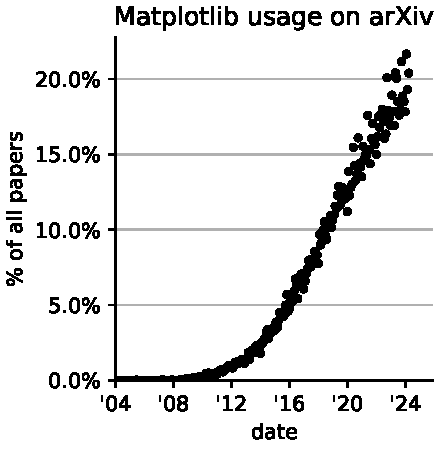
\includegraphics[width=0.45\textwidth]{arXiv_usage}
  \caption{\small Percent of uploaded papers on arXiv per-month that have a Matplotlib
    metadata in the files associated with the paper.  The percent of papers
    \texttt{astro-ph} categories is shown as black squares while
    the percent of all papers is shown as gray circles.}
  \label{fig:arxiv}
\end{wrapfigure}


% We expect that a large fraction of NASA SMD-sponsored projects rely on this
% shared infrastructure to some degree, but this is hard to quantify.  It is not
% usual, but becoming more common, to cite tool chains in scientific literature,
% so citation counts are likely to under-represent the scientific use of
% Matplotlib.  Nevertheless,
The canonical reference for
Matplotlib~\cite{Hunter:2007} has between 12,800~\cite{ads_mpl} and
32,700~\cite{gs_cites} citations depending on what works are indexed.  A direct
way to measure Matplotlib usage in scientific papers is to look at the files
uploaded to the arXiv~\cite{arxiv_stats}.  When saving figures Matplotlib
inserts a string into the file metadata indicating that it was created by
Matplotlib (and by what version).  By searching the files uploaded to the arXiv
for the string \texttt{'matplotlib'} we can put a lower bound
%, as
%post-processing may lose the metadata,
on the number of papers that mention or have at least one figure generated by
Matplotlib -- either directly or via a more specialized library.  As shown in
Figure~\ref{fig:arxiv} Matplotlib has seen steady adoption in the astronomy
related categories specifically and across arXiv generally.  As of early 2024
over 50\% of new papers uploaded in the \texttt{astro-ph} categories -- and
20\% across all categories -- have used Matplotlib.

\textbf{All measures of Matplotlib's usage show clear upward trends indicating the
growing reliance on Matplotlib by the scientific community.}

% - update with more recent examples, sort by division
These measures show broad impact but cover many uses outside of the
SMD community.  Several highlights showing where Matplotlib is used
to study galaxy evolution~\cite{2022ApJ...940L..14N} with JWST,
to study exoplanets~\cite{2020AJ....160..116G, Barclay_2018,2019AJ....158...27L} with TESS,
to study the outer solar system~\cite{Emran_2023},
to study the sun [NEED CITE],
for Martian studies~\cite{2022JE007697} and planning Rover drives at JPL~\cite{acurtis},
for lunar studies~\cite{NESNAS2023163},
and to study the Earth~\cite{paolo_2024}.
    % https://github.com/nsidc/NSIDC-Data-Tutorials <- cartopy + direct Matplotlib
This list shows the breadth of Matplotlib usage across the Astrophysics,
Planetary Science, Heliophysics, and Earth Science divisions of SMD.
Maintaining Matplotlib's health and engineering for its future will
have wide-ranging impacts for the scientific community, and for NASA in
particular.
%It has been used in tens of thousands of
%academic papers, plotting for news and sporting media, technical
%dash-boarding, and most modern data science applications.
Matplotlib falls under the umbrella of projects which the National Academies of
Science recommended for funding in the report ``Open Source Software Policy
Options for NASA Earth and Space Sciences (2018)''~\cite{NAP25217} (Option B4).
As shown above the usage of Matplotlib has only increased in the six years from
that report.  \textbf{Investments in Matplotlib will have returns across the
  entire SMD portfolio}.

% - TODO do we have any new really high-profile examples?
% Matplotlib has been used in a number
% of high-profile astronomy projects including the Nobel prize-winning
% observation of black hole merger by the Laser Interferometer
% Gravitational-Wave Observatory (LIGO), the 2020 Nobel prize-winning
% discovery of a super massive compact object at the center of our
% galaxy and the recent observation of Sagittarius A* by the Event
% Horizon Telescope (EHT).

Arranging direct meetings with NASA missions, centers, and data repositories
will produce very localized but very high-value impact.  A few hours of
consultation could save mission scientists days of figuring out how to do
something, due to the Matplotlib team's expertise in the visualization
libraries.  In particular, we expect to provide advice on how to use new
developments, including on-going refactoring under a previous ROSES award as
discussed above and the new development resulting from this award, and how to
use the libraries as efficiently as possible.  In cases where the libraries do
not yet meet the needs of the missions we use collected feedback to prioritize
development under this grant, ensuring that the libraries are responsive to the
needs of SMD researchers and engineers.

This proposal continues the path to Matplotlib's sustainability, and provides the means to
move Matplotlib forward.  Over the past 4 years, with funding from CZI and NASA, we have
shown the benefit of having paid developers.
Given the usage and the scale of
the library it is not sustainable to return to maintaining Matplotlib as a
volunteer-only effort.  A core team of full-time developers and managers can
better coordinate and nurture volunteer efforts, with the goal of growing and
sustaining a diverse community of volunteer expert contributors.

%TODO: GML: These following paragraph overlaps with the one above, I think we can cut the one below here
% With explicit support for their time, Matplotlib's core developers
% will better be able to plan the project's future.  This requires vision,
% coordination with the rest of the scientific Python community, including
% downstream libraries, and getting out in the community to get feedback.  It is
% very hard to provide that leadership and vision while working on the project during
% ``nights and weekends''.

\subsection{Technical Approach and Methodology}


\subsubsection{Consultation Services}

We will offer dedicated time to consult with NASA missions, centers, and data
repositories on usage of Matplotlib and Cartopy.  These will be structured as
virtual meetings between supported members of the Matplotlib and Cartopy teams
and representatives of individual NASA missions, center, or data repository.
The agenda of these calls will be relatively open with the goal of
understanding the unmet needs of the missions.  In some cases we expect to be
able to assist the missions to better use the existing tools to address their
needs, but in other cases we expect these discussions to drive new development
in either supported library.  This will feedback into our maintenance efforts,
highlighting areas for improvements in documentation and providing context to
new feature development.  In planning for this grant we have had early
conversations with NASA-ISRO SAR (NISAR) and Geospace Dynamics Constellation
(GDC), which were productive and point to this being generally useful.


We plan to run these consultations approximately twice a month -- which over
the lifetime of the grant should allow us to meet with representatives of up to
120 missions -- but will adjust based on demand.  The initial meetings will be
set by leveraging existing professional relationships to identify interested
missions.  We will develop an outreach plan to disseminate the existence of
this effort to the broader SMD community.



\subsubsection{General Maintenance}

Matplotlib is a primarily community-driven project, but we have grown to the
point where we need supported developers with the time to organize, plan, and
make decisions.  Supported developers will continue to allow us to take on more
complex projects than can be implemented by part-time volunteer effort alone,
while executing critical day-to-day maintenance tasks required to keep the
project healthy.


We need to sustain Matplotlib as a vibrant project and continue to support the
hundreds of thousands of users and hundreds of downstream packages.  To maintain
Matplotlib's health we must:
\begin{itemize}[noitemsep]
\item fix critical bugs and regressions promptly as they are reported;
\item entrain new contributors to sustain and diversify the community
  developer team;
\item make improvements while maintaining backward compatibility and
  documenting changes;
\item categorize Issues and PRs in terms of topic, difficulty, and
  urgency;
\item maintain the continuous-integration infrastructure;
\item manage the release process;
\item and manage community discussions about proposed enhancements, features,
  and API changes.
\end{itemize}
These are tasks that are never ``done''; users find new ways to use the
library, they expose previously un-detected bugs, they request or propose new
features, and the world continues to changes around us.  This scope also covers
small-to-medium development of new features that are opportunistically
identified.  \textbf{Dedicated full-time developers help ensure that things
  happen in a consistent and timely manner, and provide the crucial roadmaps
  that will steer the future of the library}.


% Historically, pull requests (PRs) and issues have been submitted
% faster than they can be reviewed; Matplotlib has accumulated about 300
% open PRs and 1300 open issues due to this imbalance. There are
% critical bug reports and insightful feature requests among the issue
% backlog, while among the PR backlog there are useful contributions or
% bug fixes that would improve the library for direct users and
% downstream packages.  The large backlog is discouraging for new and
% occasional contributors and distracting for core developers.

% - TODO update to include rest of CZI grants + current ROSES grant
In 2020, with a grant from CZI supporting a Research Software Engineer
(RSE) working on Matplotlib for 10 month, we resolved 2,056 PRs and
999 issues.  However, even at this rate we only reduced the PR backlog
by 70 open PRs and held the issue backlog even.  As part of reducing
the backlog, we were able to fix several long-standing bugs.  We have
demonstrated that supporting maintenance work has a positive effect on
the health of the project and \textbf{the additional resources
  requested here will further reduce, but not eliminate, the
  maintenance backlog}.


%TODO: Move some of the technical content from the objectives section to here
% where we can talk about technical details of how you'll execute the plan
% to complete the objective

\subsubsection{Cartopy Refactor}

The Cartopy refactor will be a multi-step process that will involve updating the
Cartopy codebase to take advantage of the new Matplotlib data model. This will
involve updating the Cartopy transform stack to use the new Matplotlib transforms
and data structures. Additionally, we will update the Cartopy documentation to
reflect these changes and provide new examples that demonstrate the performance
improvements and new features that are possible with the new data model. We will
also work on improving the performance of the underlying geographic transforms within Cartopy
by reducing the number of calls to the underlying projection library and optimizing
the transform stack to cache intermediate results where possible. All of these items
can be broken up into smaller PRs that can be reviewed and merged incrementally providing
a way to keep progress on the grant moving forward and not become blocked on a single
large PR/idea that may take longer to implement. The two specific features that we are
focusing on enhancing with the work in this proposal are tile sources and path transformations.

\paragraph{Tile Sources}

Tile sources are a way to display map data that is
tiled at different zoom levels to provide a more detailed view of the map as the user zooms
in. Map tiles are essentially small images that, when assembled, create a seamless map at
different zoom levels and locations. These tiles are often fetched from online servers
that provide map imagery, such as NASA, USGS, OpenStreetMap or other commercial map providers,
allowing users to visualize geographic data overlaid on detailed base maps.

Currently, Cartopy has a \texttt{SlippyImageArtist} class that is responsible for handling the
logistics of requesting these tiles. It calculates which tiles are needed based on the
map's extent and zoom level, makes requests to the tile server, and assembles the retrieved
tiles into a cohesive map. This functionality is crucial for users who need to overlay geospatial
data on top of dynamic and high-resolution basemaps, enhancing the clarity and context of
their visualizations.

However, the current implementation of \texttt{SlippyImageArtist} can be improved by leveraging
Matplotlib's new data model. This refactoring would allow the class to automatically determine
the tile scale and dimensions required for any given map projection and zoom level. By integrating
with Matplotlib's data model, \texttt{SlippyImageArtist} can become more efficient and accurate in
its tile requests, reducing redundancy and improving performance.

With an automated tile source system, Cartopy will become more accessible to a broader range of
scientists and researchers who rely on high-quality maps for their work without them having to learn
a complicated API or manually manage the tile requests. This can also be a great example use-case for other
downstream libraries to follow when integrating with the new Matplotlib data model.

\paragraph{Path Transformations}

The second area of focus for the Cartopy refactor is in the handling of path transformations from
one projection to another. In Cartopy, transforming paths from one map projection to another can
sometimes result in visually unappealing artifacts or loss of detail,
especially along curved lines and coastlines. This is due to the insufficient
number of points used to represent the path, leading to jagged edges or inaccurate
representations in the target projection.
Figure~\ref{fig:cartopy_interpolation} shows an example of the current subsampling technique
used in Cartopy that produces some unwanted representations.
The red line is a geodetic path from Japan to California, while the blue line
is the same path but reversed going from California to Japan. The current subsampling technique
uses a fixed threshold to determine whether chosen points provide a small enough angle indicating
it is a "smooth enough" curve. The default fixed threshold is not always appropriate for all
paths as shown in the figure where we'd want to visually see a smooth path (dashed black line) and not two distinct lines.

\begin{wrapfigure}{l}{0.5\textwidth}
  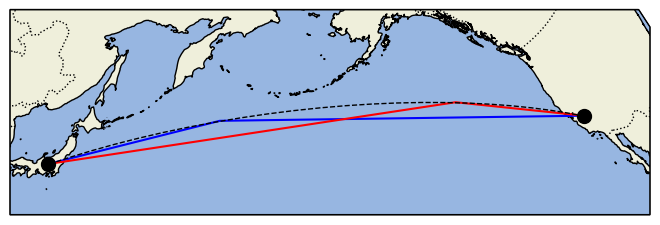
\includegraphics[width=0.45\textwidth]{supplemental/cartopy_interpolation}
  \caption{\small Example geodetic path from Japan to California demonstrating
  that the default threshold is currently too large in some cases. Additionally,
  the line from Japan to California (red) is not the same as the line from
  California to Japan (blue) due to the current subsampling technique.}
  \label{fig:cartopy_interpolation}
\end{wrapfigure}


To address this, we propose implementing an adaptive path subsampling technique similar to
the one used in the D3 JavaScript library. This method ensures that additional points are
added along the path, preserving the smooth curvature and detail during the
transformation between projections. The smoothness required for a curve will depend on the current
zoom level when rendering which we will be able to leverage the new Matplotlib data model for easily
accessing the current data limits and requirements on rendering. The proposed method also ensures that
the direction between the paths from
A->B or B->A produce the same result and we don't have the situation with the blue and red curves
shown in the figure where different users may get different results depending on the order of their data.
% Links for future reference:
% https://observablehq.com/@d3/adaptive-sampling
% https://bost.ocks.org/mike/simplify/
% Douglas-Peucker algorithm, Visvalingam’s algorithm, and Reumann-Witkam algorithm
% https://algorithm-wiki.csail.mit.edu/wiki/Line_Simplification


The adaptive sampling algorithm operates by recursively subdividing path segments,
adding points where the curvature is high and fewer where it is low.
This technique is essentially the inverse of line simplification algorithms,
which reduce the number of points in a path while retaining its overall shape.
In adaptive sampling, the goal is to increase the number of points, enhancing the
fidelity of the path in the target projection. The algorithm works by evaluating
the distance between the path's original line segments and the straight line
connecting the endpoints in the target projection. If this distance exceeds a
certain threshold, a midpoint is added, and the process repeats recursively until
the desired level of detail is achieved.

Implementing this in Cartopy involves integrating a recursive function that checks
each segment of a path during the transformation process. For each segment, the
function calculates the distance of the segment from the straight line connecting
its endpoints. If the distance is greater than a predefined tolerance, the algorithm
adds a new point at the midpoint of the segment. This new point is then used to further subdivide
the segment. By doing so, the algorithm dynamically adjusts the density of points along the path,
ensuring smooth transitions and accurate representations in the target projection.
This adaptive approach not only enhances the visual quality of transformed paths
but also improves the accuracy of spatial data analysis and visualization in Cartopy.

\subsubsection{Matplotlib Enhancements}

Ticks and tick labels are a fundamental part of what differentiates a
visualization from an illustration and allow the viewer to extract quantitative
information from the figure.  To this end Matplotlib has extensive and flexible
machinery for place and labeling ticks.  However, this flexibility comes at a
performance cost, the current design architecturally prevents hierarchical
labeling, and reduces API usability by making some seemingly simple tasks
surprisingly complex. Although we have had discussion about these issues since
at least 2015, it has been intractable to make significant progress with
volunteer effort alone.


Currently each individual each individual ``tick''
represents the union of a single tick label, tick, and grid line.  For
figures that have many axes simply creating the individual objects required
to represent all of the ticks can be a significant performance bottle neck.
Because each tick is independent it makes in extremely difficult to place a label
between, rather than at, ticks.  Finally, the current implementation only supports
two levels of ticks and tick labels (major and minor) cases where three or more layers --
such as labeling year, month, and day -- require significant work to achieve.

To address this we propose two changes to the library.  First, we will use
three collections -- for the tick labels, the ticks, and the grid lines --
essentially transposing the representation which will greatly reduce the
overhead at creation time and enable use to leverage more efficient drawing
routines already in the library to speed up rendering.  Additionally, by
representing all of the tick labels together it will be possible to implement
labeling ``between'' ticks rather than ``at'' ticks because we will have access
to the positions of more than one tick at draw time.
The second is to generalize
the current two level system to an arbitrary number of levels.

While the work to design the new API is significant, our primary concern will
be to complete this work while minimizing the impact on existing users.
Because tick labeling is so fundamental to plotting, even small changes to the
API will have significant impact on our users.  Along with the code we will
develop completed documentation of the new system, including a migration guide.


Similar to ticks, legends are another fundamental component of data
visualization where the API in Matplotlib is both very flexible but still has
an architectural limitation we plan to address.  Matplotlib has functionality
to automatically generate a legend based on what is plotted in the figure.
Generating a legend is as simple as providing a string label when plotting and
then calling a single method.  However, the configuration of how to generate
the legend entries automatically is in an external registry which is not
discoverable and complicated to modify.  Further, the machinery assumes that
each \texttt{Artist} will only need to put a single entry in the legend.  This
is already not true in some scatter
plots\ \footnote{\url{https://matplotlib.org/stable/gallery/lines_bars_and_markers/scatter_with_legend.html\#automated-legend-creation}}. and
is likely to become a bigger problem going forward as we expect to begin
generating additional composite \texttt{Artist}s.


We propose to make two changes to how legend are automatically generated: first
to move the generation of the legend entry from an external registry to a
method on each \texttt{Artist} and second to extend the API of that method to
allow the return of multiple legend entries rather than a single entry.  By
putting the code to generate the legend entry on the \texttt{Artist} we will
increase the locality of the code, make it easier to override the default, and
make it possible to ensure legend entries are updated to stay in-sync with any
style changes to the \texttt{Artist} the refer to.  The second change will
allow support for \texttt{Artist} to trivial participate in the standard automatic
legend support.

As with the work on ticking described above, the technical implementation is not
challenging, however ensuring that we have covered all of the use cases of the current
implementation and back-compatilibilty for our users.  The same as the tick work described above
we will generate completed documentation of the new system including a migration guide.

We expect that through the consultations we will be able to identify several
similar scale projects that directly address the needs of one or more NASA
mission.

\subsection{Risk Management}

There is minimal risk in the maintenance work.  There is a large volume
of individually small tasks that need to be addressed: the issue and
PR backlogs.  Any dedicated effort devoted to clearing the backlog
will have a positive impact on the project.  We have demonstrated that
supporting developers for maintenance work is an effective and
efficient use of resources.

% risk is discrete event that would cause grant to fail

There is personnel risk in that we have not yet identified the second RSEs who
will be a key individual for carrying out this work.  We are optimistic that we
will be able to recruit a qualified individuals in reasonable time.  We have
now hired two individuals as fulltime RSEs through NumFOCUS within reasonable
time frames and have almost 5 years of experience managing and paying
Research Software Engineers through NumFOCUS.


Within the Cartopy refactor, the primary risk is that the new Matplotlib data
model may not be as beneficial as we anticipate or not provide the necessary
functionality to support the new features we are planning to implement. This is
a minor risk as we have been involved in the development of the new data model
and can push changes upstream to the Matplotlib codebase if necessary.
The proposed adaptive resampling technique for path transformations may also
present challenges in terms of implementation and performance. The algorithm
is non-trivial when moving between different projections and may require additional
thought and testing to ensure that it works correctly in all cases.
However, Dr.\ Lucas has an experimental branch where he has tried some of these
techniques with some success and we are confident that we can implement this
feature in Cartopy.

We may find that refactoring the ticking system is more technically challenging
than we expect.  However, we have significant experience in the project, we
recently completed a similar but smaller scale refactor with minimal user
disruption, and have well established process Matplotlib for communicating
deprecations to the user.  Ideally we will be able to switch to a more
efficient implementation in a way that is transparent to the user, if this proves
intractable we will provide the more efficient implementation as an opt-in feature
available to users.

% TODO TAC: I am not 100% sure why we have this section, inherited it from
% last years
% GML: In other proposals I've submitted I generally have a "management structure" section
% similar to this, but it is much shorter just indicating "TAC has extensive experience
% and will lead effort X, GML has experience with Y and will lead effort Z". If we need
% to cut text I think we could consolidate some of this, but IMO it is important to indicate
% who will be in charge of what tasks and that we've thought it through and have the
% know how to successfully do this project.
% Eric agreed this was an odd section.  I think I templated this from a propsoal that was
% making the case why that team was the right team for the project out of a bunch of
% similar teams.  comment out for now, agree the that the responsibilities need to be covered
% somewhere else.

% \subsection{Contributions of Principal Investigator and Key Personnel}
%
% Dr.\ Thomas A.\ Caswell has the sole individual responsibility for directing
% and supervising the execution of this work.  He has extensive experience
% developing and maintaining Python libraries for scientists.  He has been
% involved with Matplotlib from 2012 and had a leadership role in the project
% from 2014.  He is also a core developer of h5py and has contributed to many of
% the other core projects of the SPE.  He is currently a group leader of the Data
% Acquisition and Detectors group in the Data Science and Systems Integration
% program at the National Synchrotron Light Source II (NSLS-II) at Brookhaven
% National Labratory and the technical lead of a new beamline at NSLS-II.  He is
% also the lead architect and developer of the Bluesky Suite, an ecosystem of
% co-developed libraries and applications for data acquisition and management,
% which is being adopted for beamline operations at synchrotrons in the US and
% across the world.
%
% Dr.\ Greg Lucas is currently a maintainer of both Matplotlib and Cartopy.
% He will lead the integration of the new Matplotlib Data Model into the Cartopy package.
% He will be updating documentation, adding new examples, and improving the performance of
% the geographic transforms within Cartopy as a part of this work. He has experience
% with the transform stack of both Matplotlib and Cartopy, including a major refactor
% of the Cartopy transform stack to switch to using the pyproj library. He is currently
% the Science Data Center lead for the Interstellar Mapping and Acceleration Probe (IMAP)
% at the Laboratory for Atmospheric and Space Physics (LASP) managing a science data
% processing team working directly with NASA mission data. He is an open-science advocate
% and is NASA TOPS certified.
%
% Dr.\ Kyle Sunden will be the primary developer for the improvements to Matplotlib.
% This includes the ticker refactor and making Matplotlib figures more sharable.
% In addition, Dr.\ Sunden will perform maintenance for Matplotlib.
% Maintenance encompasses reviewing and responding to incoming pull reqests and issues, fixing known bugs, and smaller feature development tasks.
% As an active member of the development team, Dr.\ Sunden will participate in planning discussions regarding future improvements to the library.
% Finally, maintenance also includes interfacing with both upstream and downstream scientific python projects to ensure continued interoperability.
% Dr.\ Sunden will also participate in community building for the project.
% He will participate in the majority of the consultation sessions provided to NASA funded Missions.
% He will mentor new contributors, including participation with the Google Summer of Code project.
% Finally, Dr.\ Sunden will attend events such as the SciPy Conference and Scientific Python Developer Summit, where he will engage in high bandwith discussions with maintainers of related projects and users of Matplotlib.
% This will include presentations and/or tutorial sessions at these events.

\subsection{Work Plan}

We also plan to split the effort 75\% / 25\% between
Matplotlib and Cartopy.  For Matplotlib we plan to split the effort on this
grant 65\% / 20\% / 15\% between maintenance, new development, and community
engagement and community and project management.  We intend to target this distribution
of effort across the lifetime of the grant, but there may be variations year-to-year.
% This is (for Matplotlib over 5 years)
%  maint: 5.85 FTE
%  new feature: 1.8 FTE
%  community: 1.35 FTE + .1*5
For Cartopy, the proposed split in effort will be roughly 30\% / 60\% / 10\%
between maintenance, new development, and community engagement and community
and project management.  We plan to focus more on new development efforts and
integrating the new Matplotlib data model which will take a fair amount of
effort to develop the proper transforms and data structures to take advantage
of the new data model.


\subsubsection{General Maintenance}

Throughout the project both Dr.\ Caswell, Dr.\ Sunden, Dr.\ Lucas, and the RSE
will work on general maintenance and community engagement of both Matplotlib
and Cartopy.  This includes, but is not limited to, fixing bugs, reviewing Pull
Requests, answering user questions, managing releases, and welcoming new
contributors to the project.


\subsubsection{Cartopy Refactor}

The Cartopy refactor will begin at the start of the grant period
and the work effort will be evenly split across all years in the grant.
During the first two years of the grant there will be an emphasis on
integrating the new Matplotlib data model into the Cartopy codebase.
The third and fourth years will focus on implementing the specific
features of tile sources and path transformations utilizing the new
Matplotlib data model as appropriate. The final year will be spent on
improving the performance of the methods. Throughout the grant, general
maintenance and community work will be performed in parallel with the
explicit Cartopy refactor tasks.


\subsubsection{Ticker Refactor}

The Ticker refactor will begin at the start of the grant period, Y1Q1 and will take place over the course of 18 months, in parallel with general maintenance and community work.
The initial quarter will focus on planning and API design for the new ticking system.
This will include gathering examples of plots which could take advantage of the new ticking system.
The technical implementation of the new ticking system will primarily take place in Y1Q2, with testing and documentation following in Y1Q3.
It is expected that the design and integration with existing APIs will be a significant portion of the total effort.
The initial release as an opt-in feature will be in Y1Q4.
This will be followed by bug fixes and additional integration of pre-existing APIs.
We expect to be ready for full release in Y2Q2, though may opt to delay for one or two more releases to allow additional time for feedback from our users.

% Y1Q1: Planning and Design
% Y1Q2: Implementation
% Y1Q3: Testing and Documentation
% Y1Q4: Initial release as opt-in behavior
% Y2Q1: Bug fixes and integration
% Y2Q2: Release as default

% \subsubsection{Sharing Figures: Serialization}
%
% Following the conclusion of the Ticker refactor, another 18 month cycle will focus on the first portion of the sharing figures project, namely a serialization standard for Matplotlib figures.
% The first quarter (Y2Q3) will be primarily focused on planning and design requirements, with small proof of concept developement tasks.
% The second quarter (Y2Q4) will focus on serializing the Matplotlib \texttt{Artist}s and their relationships.
% The third quarter (Y3Q1) will in particular extend that work from the previous ROSES award, allowing serialization of both Data Containers and the transformation pipeline.
% It is expected that data serialization will be of particular technological consideration, as some Data Containers contain large amounts of data and/or reference data hosted in other locations (e.g. local files or remote web services).
% Following thourough documentation and testing, we expect a release to be available in Y3Q3, after which most effort will be in responding to user feedback and interfacing with downstream libraries to disseminate the work.
% % Y2Q3: Planning and Design
% % Y2Q4: Implementation serializing Artist tree
% % Y3Q1: Implementation serializing Data containers and transformation pipeline
% % Y3Q2: Documentation and testing
% % Y3Q3: Release, respond to user feedback
% % Y3Q4: Bug fexes and use cases
%
% \subsubsection{Sharing Figures: Bundling}
%
% The last major feature enhancement to Matplotlib is to create a standardized bundle for sharing fully functional, interactive figures.
% The goal is to have statically distrubutable assets that provide a Python runtime, dependencies, and allow a web browser to display the figures.
% This will be built heavily on top of the serialization efforts described above.
% This portion of the figure sharing project relies on upstream libraries, including Pyodide.
% As this project is not anticipated to be started until year 4 of the award, a significant step will be to survey the available libraries, which could easily have changed by that time.
% As such, the first quarter (Y4Q1) will focus on a technilogical survey of existing technologies and their comparitive suitability for providing a bundled python runtime, dependencies, and graphical user interface.
% The following four quarters (Y4Q2-Y5Q2) will conist of the active planning, implementation, documentation and testing.
% This will culminate in the initial feature release in Y5Q2.
% To mitigate risk and avoid unnecessarily adding dependencies for users who do not need this feature, it will be released as a separately installable package, rather than integrated into the main Matplotlib codebase.
%
% % Y4Q1: Survey of upstream library options
% % Y4Q2: Planning and Design
% % Y4Q3: Implementation
% % Y4Q4: Implementation
% % Y5Q1: Documentation and Testing
% % Y5Q2: Release and Bug fixes
%
\subsubsection{Work Process}

All work under this proposal will undergo the same review process
as any other contribution.  We
encourage many small PRs to reduce risk.  At least one maintainer not
supported on this proposal
will need to sign off on any changes before they are merged. This
disseminates understanding of the proposed work and ensures
community buy-in.  Finally, by merging
changes to the default branch continuously throughout the period of
work the incremental improvements will be released as part of our
semiannual release cadence.

The RSE will present the status of the work at two conferences yearly,
expected to be SciPy in July and one of PyData regional conferences in
the winter.


\subsubsection{Grant Management}

Dr.\ Caswell of BNL and the Matplotlib Project Lead is the PI of the proposed
development.  He is responsible for the quality and direction of the proposed
work and the proper use of all awarded funds.  He is also responsible for all
management, and budget issues and is the final authority for this task.

Dr.\ Lucas of UC Boulder is the institutional PI for UC Boulder and is
responsible for the Carotpy work including the proposed refactor.


\subsection{Matplotlib and Cartopy Project Management}
\subsubsection{Governance and Finances}

Matplotlib is a NumFOCUS Fiscally Sponsored Project.

From 2020 onward Matplotlib is governed by a steering council, a Project Lead
(PL), and several Deputy Project Leads (DPL)~\cite{gov}.  The current PL is
Dr.\ Caswell.  We are a community project and try to make all decisions, both
strategic and day-to-day, by consensus.  However, if consensus can not be
reached, the responsibility falls back to the DPLs and ultimately to the
PL.\footnote{Prior to 2020 Matplotlib used a ``BDFL'' model lead by Dr.\ John
Hunter until 2012, Dr.\ Michael Droettboom from 2012-2014, jointly by
Dr.\ Caswell and Dr.\ Droettboom from 2014-2016, and by Dr.\ Caswell from
2016-2020.}

% TODO need cartopy governance

\subsubsection{License}

Matplotlib is licensed under the Matplotlib License~\cite{mpl_lic} which is a
derivative of the Python Software Foundation license~\cite{psf_lic}.  It is a
permissive license compatible with the BSD-3 clause
license~\cite{jdh_bsd_opinions}.  Matplotlib includes several components which
are individually licensed under BSD-3 clause compatible licenses.

Cartopy is licensed under the BSD-3 clause.


\subsubsection{Sustainability Metrics}

There are many possible ways to measure the sustainability of an
open source project.  We propose to focus on growing our developer
community, reducing our Issue and PR backlogs, and maintaining a
regular release cadence.

Matplotlib is a community driven project with a majority of the
work done by volunteers.  The thing we are shortest on is the time of
maintainers who are able and willing to review Pull Requests.
Increasing the number of regular contributors and maintainers improves
the sustainability of the project in several ways; many hands make
light work and it makes the project resilient to individuals leaving
the project.

The first metric is the volume of work done.  Although quantitatively
evaluating maintenance work can be tricky --- some Issues or PRs take minutes
to review while others can take days to weeks of effort --- but we believe that
there is value at looking at the rate and promptness with which they are
addressed.  We will aim to hit the following metrics:
\begin{itemize}[noitemsep]
\item Initial response to all issues / new PRs within a week  % general responsiveness
\item Close or merge a majority of new PRs within 1 month     % improve contributor experience
  % 3mo/quarter*4wk/mo*((((5.85 total FTE for maint over grant  *.3 fraction for review) / 5 years)*40 hr/week) / 2 [hr/issue or PR])
  % -> 84 reviews / quarter
\item Resolve 80 issues to Matplotlib / quarter by supported developers       % numbers we can hit with grant labor only
\item Review and merge 80 PRs to Matplotlib / quarter by supported developers % numbers we can hit with grant labor only
\end{itemize}

The second metric we will track is the rate at which we are able to on board
new regular contributers to the project.  Historically over the past 5 years we
have average 45-55 PRs from first-time contributors per quarter of which 30-40
are eventually merged.  Of contributors with at least one merged PR, about 29\%
have 2 or more merged PRs, but of contributors who have at least 2 merged PRs
about 59\% have 3 or more.  As we consider the larger numbers of merged PRs,
the odds of someone with N merged PRs having N+1 continues to improve
approaches 90\% above 5 merged PRs.  We will aim to increase the number of
first time contributors with merged PRs by 5 per quarter, to increase the
fraction who go on to have a second per to 40\%, and to on board 2 new
core-maintainers with commit rights per year.

Finally, for the user community to benefit from our work we need to do
regular releases.  We will continue to maintain a bi-yearly release
cycle for feature releases with 1-3 bug-fix releases as needed.
Holding to a time-based release schedule is advantageous because it
provides predictability to our users and reduces the lag between when a
new feature is merged to the default branch and when it is generally
available.

% TODO something about cartopy here?

\subsubsection{Collaboration with Related Projects}


Much of the communication is through the standard communication channels, such
as project issue trackers, mailing lists or discussions forums, and submitting
PRs.  For example P. L. Lim, who is a Senior Software Engineer in the Data
Analysis Tools Branch at the Space Telescope Science Institute and Astropy
contributor regularly reports bugs to Matplotlib when pre-release versions of
Matplotlib have an impact on Astropy.  The strongest relationships, both
historical and current, are with projects where we have shared developers.
% should not use cartopy as an example of
%For
%example Greg Lucas, Ruth Comer, and Elliot sales de Andre are core contributors
%to Matplotlib and Cartopy while
For example Ryan May is an maintainer of both Matplotlib and Metpy and David
Stansby is a maintainer on both Matplotlib and \texttt{SunPy}Through NumFOCUS
and domain-specific conferences, there are regular in-person meetings between
developers.

We also regularly communicate with our upstream dependencies.  As Numpy
prepared for a 2.0 release we were in constant communication to ensure that we
were able to smoothly support users through the upgrade.  One of the flagship
new features in Python 3.13 is a re-implemneted prompt.  When we brought to the
CPython developers attention that it was missing a feature of the old prompt it
was promptly addressed and considered a blocking issue for beta2.

% wording all NF projects are putting in, please avoid wordsmithing it.
As a NumFOCUS project, we recognize the importance of every project
that is part of our open source scientific computing community. Though
we would like for our work to be funded we are committed to supporting
and collaborating with other NumFOCUS projects that receive funding
regardless of our own outcome. We believe that this attitude is
crucial for the success of our community and the sustainability of
open source projects. It is our hope that this sentiment will be taken
into consideration when evaluating our proposal.


\subsubsection{Inclusive Community Development}

% - TODO this subsubsection may move to the inclusion plan which is
% required for foundation level call
% GML: I agree to move this into the inclusion plan. I think this is a
% strong case and well written. We can add a sentence or two within the
% main proposal that references out to this text in the inclusion plan.
% TAC: my concern with moving too much to the inclusion plan is that
% it listed as a pilot part of the popsoal that will not affect if
% we are awarded or not so I am not sure if the it will be reviewed by
% the main panel or a separate panel that only provides feedback on the
% inclusion plan.

Matplotlib strives to be an inclusive and open project, anyone who is
willing and able to contribute to the project should feel welcome to
do so.  We have adopted the Contributor Covenant V2.0 as
our Code of Conduct~\cite{CoC}.

Matplotlib has an open development model, all work is done in the open and
welcome contributions, in the from of bug reports, feature requests, or pull
requests from anyone.  We maintain an extensive contribution guide
(\url{https://matplotlib.org/devdocs/devel/index.html}) as part of our
documentation.  To improve the development and retention of new contributors we
run two efforts: an ``incubator'' channel on gitter and bi-monthly New
Contributor calls.

%% I really want to put this in, but do not see a good place for it :/
% It is important for everyone working on the project to feel safe to make
% mistakes.
% GML: I agree with this sentiment. I wonder if we can put something in about
% the project being OK with reverting commits. I actually had an experience in
% numpy that was kind of funny with having a large-ish PR merged two times and
% reverted both times because of downstream breakages. But, it was very nice that
% they were willing to merge and revert and not really a big issue IMO.

We strive to maintain a developer community where everyone feels safe to make
mistakes. Everyone makes mistakes and almost all code written alone can be
improved by working together.  We have processes in place -- code review,
automated tests, and publishing release candidates -- to catch those mistakes
before they reach our users.  Feedback during review should be delivered with
compassion and professionalism and everyone working on the project, independent
of their tenure with the project or seniority outside of the project, needs to
open continued learning and improvement.



The hardest part of getting started to contributing to open source
projects is simply figuring out where and how to begin.  Open source communities,
particularly big ones, can be intimidating for first time
contributors.  The incubator is a semi-closed chat room where new
contributors can get support on any aspect of contributing to
Matplotlib.  This includes the technical aspects of the code they are
working on, help with git/GitHub, our review process, or the social
expectations and norms of the community.  The goal is that by
providing this support to first time contributors we will retain more
of them as regular contributors and then maintainers.

The issue tracker is important to communication on the project because
it serves as the centralized location for making feature requests,
reporting bugs, identifying major projects to work on, and discussing
priorities.  For this reason, it is important to curate the issue
list, adding labels to issues and closing issues that are resolved or
unresolvable. Triaging issues does not require any particular
expertise in the internals of Matplotlib but is extremely valuable to
the project.  To this end we have created a ``Triage Team'' in the
organization who have power to tag, milestone, and close issues.  In
addition to the direct benefit of improving the issue triage and
freeing the core-developers to spend more time reviewing PRs, this
role will bring more people into the developer community and may
provide a pathway to becoming regular contributors and maintainers.

Ongoing work at NumFOCUS to develop metrics on new contributors
will help us evaluate the
efficacy of these efforts at diversifying our contributor base.

\subsubsection{Contribution Workflow}
%check that this is not a required title
%\subsection{Technical approach and methodology}

Matplotlib is an established community driven project in the
``federation'' model as defined by Nadia Eghbal~\cite{eghbal_2020}.
We have a core group of regular maintainers who take responsibility for
reviewing and merging proposed changes to the library and welcome Pull
Requests from anyone who is interested in contributing.  We strive
for consensus and rely on the collective judgment of our maintainers
to maintain the quality and functionality of the library.

Matplotlib uses a variation on the ``git flow'' process~\cite{ghflow}
to manage proposing and reviewing contributions to the library and
documentation on GitHub.  Changes are proposed by opening a ``Pull
Request'' on GitHub; the process is the same for core maintainers,
regular contributors, and a first time contributor.  The proposed
changes are reviewed by maintainers who either request changes, which
starts a cycle of iteration with the contributor, or approve.  In
addition to human review we have an extensive test suite that is
automatically run via cloud services and reported to
the PR.  Once consensus is reached, documentation is written,
and the tests pass the PR is merged.  The changes are made widely available
as part of the next release.

Matplotlib maintains an extensive suite of automated tests that
exercises a large fraction of our code base (>90\% code coverage).  The full test suite, and
a build of the documentation, is run against several versions of
Python on OSX, Windows, and Linux hosts on every PR and merge to the
default branch via continuous integration.  For every new feature or
bug fix that gets merged we also add tests that codify the expected
behavior.  This gives us the ability to make changes to the library
with confidence that we will not break existing behavior.

The review threshold for merging a PR depends on the risk of the changes.  PRs
that only change documentation, which cannot introduce regressions or introduce
new features, may be merged by the first reviewer whereas code changes need to
be reviewed and approved by at least two maintainers (not including the author
of the PR).  If consensus cannot be reached, the final decision falls back to a
Deputy Project Lead or the Project Lead.

Matplotlib is cautious about making backwards-incompatible change that
intentionally break users existing code.  While in an ideal world, future
versions of the library would be 100\% backwards compatible with previous
versions, sometimes we do need to make incompatible changes.  As part of the
review process we check that any API changes are well documented and justified.
When technically possible we provide user-visible warnings the version before
we actually implement a breaking change.  This provides a window for users to
either adapt to the change or to communicate to us that they cannot adapt so we
can reconsider the change.  Given this high barrier to changing or removing
behavior we are careful to make sure that any new API we add to the library is
well thought out and complete because once we have it is hard to take back or
change features once released.  These considerations together are important
enough that we have a Deputy Project Lead responsible for API consistency.

This process works well for incremental contributions and bug fixes.  Bigger
changes, such as major new features or significant refactors, are typically
discussed before significant work is done.  In many cases if a feature does not
need to be in the core library we encourage contributors to create a new
stand-alone project.  This has several advantages including giving the
author more control, allows them to iterate faster than our 6 month release
schedule, and gives them greater flexibility to change their APIs during
initial development.

\subsubsection{Information Dissemination}

As a project Matplotlib maintains a range of communication channels
aimed at several, overlapping, audiences.  This includes a
the source, issue tracker and PRs on GitHub,
the published documentation (including historical and development versions),
weekly developer call,
bi-weekly new contributor calls,
mailing lists,
a discourse forum,
a real-time chat platform (gitter),
in-person presentations and discussions at conferences and pydata events,
and several social media accounts.


The center of gravity of Matplotlib development takes place on GitHub
(\url{https://github.com/matplotlib/matplotlib}) where the canonical
repository for the source and documentation is hosted.  Around this
repository we use Issues and PRs to track bug reports, feature
requests, and to discuss proposed changes.  We also host our
governance documents on GitHub
(\url{https://github.com/matplotlib/governance}) and revise them via
Pull Request.

We publish extensive prose, example, and API documentation
(\url{https://matplotilb.org}).  We host documentation for for the most recent
version at (\url{https://matplotilb.org/stable}), historical versions for past
releases (e.g. \url{https://matplotlib.org/3.8.4} for the v3.8.4 documentation)
and development versions of the documentation
(\url{https://matplotlib.org/devdocs}).  In the first Quarter of 2024 we had
between 1.5-1.8M unique visitors a month to the documentation per a
Plausible.io site analytics.

The weekly developer calls are typically attended by six to eight people and
are used for high-bandwidth discussions about both the overall direction of the
project and technical issues.  The agenda and minutes are publicly available
(\url{https://hackmd.io/team/matplotlib}) and the calls are open to all.

For real-time chat Matplotlib maintains a Gitter/element
(\url{https://gitter.im/matplotlib/matplotlib}) chat room which we use for
general coordination and resolving minor technical discussions.  While the chat
room's history is technically persistent, we treat it as transient.  For more
in-depth discussions or anything we want a record of, we move the conversation
to GitHub, the mailing list, or discourse.

For user support and general discussion we maintain a Discourse
(\url{https://discourse.matplotlib.org}) instance.  While users have to
subscribe or register respectively to post, this forum is open to all.  We also
maintain a read-only mailing list for announcements
(\url{https://mail.python.org/mailman/listinfo/matplotlib-announce}).

Matplotlib developers have frequently attended in-person events including
SciPy, PyData regional conferences, and domain science conferences.

\newpage
% Here's how I get references.
% needed for AAS citation

\def\ref@jnl#1{{\rm#1}}

\def\aj{\ref@jnl{AJ}}                   % Astronomical Journal
\def\actaa{\ref@jnl{Acta Astron.}}      % Acta Astronomica
\def\araa{\ref@jnl{ARA\&A}}             % Annual Review of Astron and Astrophys
\def\apj{\ref@jnl{ApJ}}                 % Astrophysical Journal
\def\apjl{\ref@jnl{ApJ}}                % Astrophysical Journal, Letters
\def\apjs{\ref@jnl{ApJS}}               % Astrophysical Journal, Supplement
\def\ao{\ref@jnl{Appl.~Opt.}}           % Applied Optics
\def\apss{\ref@jnl{Ap\&SS}}             % Astrophysics and Space Science
\def\aap{\ref@jnl{A\&A}}                % Astronomy and Astrophysics
\def\aapr{\ref@jnl{A\&A~Rev.}}          % Astronomy and Astrophysics Reviews
\def\aaps{\ref@jnl{A\&AS}}              % Astronomy and Astrophysics, Supplement
\def\azh{\ref@jnl{AZh}}                 % Astronomicheskii Zhurnal
\def\baas{\ref@jnl{BAAS}}               % Bulletin of the AAS
\def\bac{\ref@jnl{Bull. astr. Inst. Czechosl.}}
                % Bulletin of the Astronomical Institutes of Czechoslovakia
\def\caa{\ref@jnl{Chinese Astron. Astrophys.}}
                % Chinese Astronomy and Astrophysics
\def\cjaa{\ref@jnl{Chinese J. Astron. Astrophys.}}
                % Chinese Journal of Astronomy and Astrophysics
\def\icarus{\ref@jnl{Icarus}}           % Icarus
\def\jcap{\ref@jnl{J. Cosmology Astropart. Phys.}}
                % Journal of Cosmology and Astroparticle Physics
\def\jrasc{\ref@jnl{JRASC}}             % Journal of the RAS of Canada
\def\memras{\ref@jnl{MmRAS}}            % Memoirs of the RAS
\def\mnras{\ref@jnl{MNRAS}}             % Monthly Notices of the RAS
\def\na{\ref@jnl{New A}}                % New Astronomy
\def\nar{\ref@jnl{New A Rev.}}          % New Astronomy Review
\def\pra{\ref@jnl{Phys.~Rev.~A}}        % Physical Review A: General Physics
\def\prb{\ref@jnl{Phys.~Rev.~B}}        % Physical Review B: Solid State
\def\prc{\ref@jnl{Phys.~Rev.~C}}        % Physical Review C
\def\prd{\ref@jnl{Phys.~Rev.~D}}        % Physical Review D
\def\pre{\ref@jnl{Phys.~Rev.~E}}        % Physical Review E
\def\prl{\ref@jnl{Phys.~Rev.~Lett.}}    % Physical Review Letters
\def\pasa{\ref@jnl{PASA}}               % Publications of the Astron. Soc. of Australia
\def\pasp{\ref@jnl{PASP}}               % Publications of the ASP
\def\pasj{\ref@jnl{PASJ}}               % Publications of the ASJ
\def\rmxaa{\ref@jnl{Rev. Mexicana Astron. Astrofis.}}%
                % Revista Mexicana de Astronomia y Astrofisica
\def\qjras{\ref@jnl{QJRAS}}             % Quarterly Journal of the RAS
\def\skytel{\ref@jnl{S\&T}}             % Sky and Telescope
\def\solphys{\ref@jnl{Sol.~Phys.}}      % Solar Physics
\def\sovast{\ref@jnl{Soviet~Ast.}}      % Soviet Astronomy
\def\ssr{\ref@jnl{Space~Sci.~Rev.}}     % Space Science Reviews
\def\zap{\ref@jnl{ZAp}}                 % Zeitschrift fuer Astrophysik
\def\nat{\ref@jnl{Nature}}              % Nature
\def\iaucirc{\ref@jnl{IAU~Circ.}}       % IAU Cirulars
\def\aplett{\ref@jnl{Astrophys.~Lett.}} % Astrophysics Letters
\def\apspr{\ref@jnl{Astrophys.~Space~Phys.~Res.}}
                % Astrophysics Space Physics Research
\def\bain{\ref@jnl{Bull.~Astron.~Inst.~Netherlands}}
                % Bulletin Astronomical Institute of the Netherlands
\def\fcp{\ref@jnl{Fund.~Cosmic~Phys.}}  % Fundamental Cosmic Physics
\def\gca{\ref@jnl{Geochim.~Cosmochim.~Acta}}   % Geochimica Cosmochimica Acta
\def\grl{\ref@jnl{Geophys.~Res.~Lett.}} % Geophysics Research Letters
\def\jcp{\ref@jnl{J.~Chem.~Phys.}}      % Journal of Chemical Physics
\def\jgr{\ref@jnl{J.~Geophys.~Res.}}    % Journal of Geophysics Research
\def\jqsrt{\ref@jnl{J.~Quant.~Spec.~Radiat.~Transf.}}
                % Journal of Quantitiative Spectroscopy and Radiative Transfer
\def\memsai{\ref@jnl{Mem.~Soc.~Astron.~Italiana}}
                % Mem. Societa Astronomica Italiana
\def\nphysa{\ref@jnl{Nucl.~Phys.~A}}   % Nuclear Physics A
\def\physrep{\ref@jnl{Phys.~Rep.}}   % Physics Reports
\def\physscr{\ref@jnl{Phys.~Scr}}   % Physica Scripta
\def\planss{\ref@jnl{Planet.~Space~Sci.}}   % Planetary Space Science
\def\procspie{\ref@jnl{Proc.~SPIE}}   % Proceedings of the SPIE

\let\astap=\aap
\let\apjlett=\apjl
\let\apjsupp=\apjs
\let\applopt=\ao

\let\oldbibsection\bibsection
\renewcommand\bibsection{\oldbibsection\setcounter{page}{1}}
\bibliography{highlight,mpl_cartopy}


\newpage

\section{Open Science and Data Management Plan}
\setcounter{page}{1}

Matplotlib and Cartopy are software libraries and do not produce any scientific
data as defined in E.1.2 that needs to be preserved.  Both are tools used to
visualize data that is acquired through other means.

Matplotlib is a community library developed in the open on GitHub.
It is released under the Matplotlib license
(\url{https://matplotlib.org/users/license.html}) which is a permissive
license that is a derivative of the PSF license
(\url{https://docs.python.org/3/license.html}) and compatible with the
BSD-3 license.  All work done on Matplotlib as part of this grant will
be done through the current workflow, will be publicly available, and
released under the same license.  Matplotlib uses git for version
control, thus every developer has the full history on their computer
which provides significant redundancy.  Tagged releases of the
software are published to PyPI (in both source and binary forms).  In
addition, Anaconada, conda-forge, macports, homebrew, and all major Linux
distributions independently build, package, and distribute Matplotlib.
Extensive User facing documentation, including install instructions
and usage guides, is built and hosted at \url{https://matplotlib.org}.

Cartopy is a community library developed in the open on GitHub.  It is released
under the BSD 3-Clause License.  All work done on Cartopy as part of this grant
will be done through the current workflow, will be publicly available, and
released under the same license.  Cartopy uses git for version control, thus
every developer has the full history on their computer which provides
significant redundancy.  Tagged releases of the software are published to PyPI
(in both source and binary forms).
In addition, Anaconada, conda-forge, and some major Linux
distributions independently build, package, and distribute Cartopy.
Extensive User facing documentation, including install instructions and usage
guides, is built and hosted at
\url{https://scitools.org.uk/cartopy/docs/latest/}.

Any new libraries created as part of the ROSES award will be developed
in the open on GitHub and will be released under a permissive license.

Any incidental work on other software packages, either upstream or
downstream of Matplotlib or Cartopy, will follow the license and development
process of those projects.

\newpage

\section{Inclusion Plan}
\setcounter{page}{1}
% 2 pages

% Inclusion is a core NASA value, as described in the NASA Administrator’s policy
% statement on Diversity, Equity, Inclusion, and Accessibility (DEIA). Additionally, Strategy
% 4.1 of the latest version of “Science 2020-2024: A Vision for Scientific Excellence”
% states: “Increase the diversity of thought and backgrounds represented across the entire
% SMD portfolio through a more inclusive environment.”
% Inclusion is defined here as the full participation, belonging, and contribution of
% organizations and individuals. Note that inclusion is distinct and different from diversity.
% Inclusion requires that all individuals can participate fully, regardless of the diversity
% dimension, do their best work, advance their career, and feel welcomed, valued,
% connected, engaged, and supported to reach their full potential. If a program element
% requires an Inclusion Plan, it shall focus on inclusion, not diversity, accessibility, or
% equity.
% Proposers shall tailor their Inclusion Plans specifically to the proposal team rather than
% to generic issues in the broader STEM community surrounding inclusion. If
% volunteers/citizen scientists are among the proposed investigators, see Section 1(i), the
% inclusion plan should apply to those team members as well. Inclusion plans should be
% distinct from, and not solely focus on, public engagement efforts.
% Proposers are encouraged to leverage institutional resources when available. However,
% the plan should not include a restatement of policies of the host institution; rather, it
% shall provide a clear discussion of how these policies connect to the proposed
% investigation and proposal team.
% The Inclusion Plan shall:
% • clearly state the goals for creating and sustaining a positive and inclusive working
% environment for the investigation team and describe activities to achieve such an
% environment;
% • identify barriers to creating a positive and inclusive working environment that are
% specific to the team carrying out the proposed investigation;
% • address ways in which the investigation team will work to attenuate or reduce
% these barriers;
% • describe roles, responsibilities, and work efforts for Inclusion Plan activities for
% team members with specific tasks in said activities;
% • include a timeline for completing or carrying out proposed activities;
% • and contain a plan for evaluating progress towards achieving the proposed
% Inclusion Plan activities or goals.
% Unless prohibited by the program element, teams may request funding for the hiring of
% experts and/or those familiar with inclusion best practices to join the team, advise on, or
% oversee the proposed Inclusion Plan efforts. Any funding requested for Inclusion Planrelated activities shall be explicitly identified and justified in the Inclusion Plan section
% and clearly identified in the proposal budget.
% See individual program elements for the required location in the proposal for Inclusion
% Plans and page limits. For programs that use dual anonymous peer review, the
% inclusion plans are generally to be anonymized, but please refer to the specific
% instructions for the program element. If institutions or partners are contributing to or
% assisting with the Inclusion Plan efforts, but they are not otherwise on the proposal
% team, then Letters of Resource Support (see Table 1) must be included after the
% Inclusion Plan references, unless otherwise specified in the program element, and do
% not count toward the page limit noted in the program element.
% The assessment of the Inclusion Plan will be based on these factors:
% ● The extent to which the Inclusion Plan provided appropriate processes and goals
% for both creating and sustaining a positive and inclusive working environment for
% the investigation team;
% ● The extent to which the Inclusion Plan demonstrated awareness of systemic
% barriers to creating inclusive working environments that are or may be specific to
% the proposal team;
% ● The extent to which the Inclusion Plan contained appropriate activities for
% equipping team members to build and maintain inclusive working environments;
% ● The extent to which the roles and responsibilities for those participating in the
% proposed activities were well described and justified;
% ROSES SoS-37
% ● The reasonableness of the proposed timeline for the proposed Inclusion Plan
% activities;
% ● The extent to which the Inclusion Plan provided reasonable and appropriate
% assessment mechanisms for measuring progress in and success of the proposed
% activities;
% ● The reasonableness of the resources requested to execute the proposed
% activities and the quality and appropriateness of the justification for these
% resources.
% The assessment of the Inclusion Plan will be led by individuals with practical and/or
% research expertise in IDEA topics.
% Feedback will be provided to proposers in a separate Inclusion Plan evaluation form.
% The assessment of the Inclusion Plan will not be part of the adjectival rating for the
% proposal and will not inform the selection of proposals.
% It is the proposal team’s responsibility to carry out the proposed activities rather than
% fully outsource them. All team members are expected to contribute to fostering an
% inclusive and positive work environment, regardless of their involvement with specific
% Inclusion Plan activities.
% The Inclusion Plan and any associated activities are expected to reflect the size of
% proposal team, scale and complexity of the proposed research project, and the available
% budget.
% Some resources and research that may be useful when formulating an Inclusion Plan,
% can be found at https://science.nasa.gov/researchers/inclusion.
% Progress in executing the investigation’s Inclusion Plan shall be described in the annual
% progress report.

Matplotlib strives to be an inclusive and open project, anyone who is willing
and able to contribute to the project should feel welcome todo so. We have
adopted the Contributor Covenant V2.0 as our Code of Conduct~\cite{CoC}.

Matplotlib has an open development model, all work is done in the open and we
welcome contributions in the from of bug reports, feature requests, or pull
requests from anyone. We maintain an extensive contribution guide
(\url{https://matplotlib.org/devdocs/devel/index.html}) as part of our
documentation. To improve the development and retention of new contributors we
have an ``incubator'' channel on gitter, which serves as a semi-closed chat
room where new contributors can get support on their first contributions.

As part of a previous project, we started hosting New Contributor Meetings
monthly, giving first-time contributors a space to ask questions and interact
with community members on a video call. In addition, we track first-time
contributors pull requests using a GitHub project, which gives these special
contributions visibility and helps prioritize reviews and interactions with new
contributors.

To better understand the needs of our community and how to engage with it, we
will also collaborate with the CSCCE to provide guidance and training on
community management and community building.

Ongoing work at NumFOCUS to develop metrics will help us evaluate the efficacy
of these efforts at diversifying our contributor base.


  \begin{itemize}
  \item  ``good first issue'' tag
  \item https://contributor-experience.org
  \item incubator
  \item GSOC participtaion
  \item welcome bot
  \item CoC
  \item CSCCE adoption
  \end{itemize}





\newpage
\section{Biographical Sketch}
\setcounter{page}{1}
\begin{center}
  \textbf{Thomas A.\ Caswell}\\
  Computational Scientist\\
  Brookhaven National Laboratory\\
  Building 741 P.O. Box 5000\\
  Upton, NY 11973-5000\\
  (631) 344-3146\\
\end{center}

\subsubsection*{Relevant Experience}
17+ years working in data intensive experimental science.  12 years of
experience contributing to Scientific Python, 10 years in leadership roles in
the open source community.  Current Project lead on Matplotlib, past release
manager and current core developer for h5py, has contributed to NumPy, Pandas,
SciPy, and IPython.  Co-developed \texttt{trackpy}, now widely used in
soft-matter physics community.  Lead architect and developer of Bluesky Suite
for data acquisition now being adopted at x-ray facilities around the world.
Brookhaven National Laboratory/NSLS-II representative on NeXus International
Advisory Committee.

\subsubsection*{Education}
Ph.D., Physics, University of Chicago \hfill 2014\\
M.S., Physics, University of Chicago \hfill 2008\\
B.A., Physics, Mathematics, Cornell University \hfill 2007

\subsubsection*{Professional Experience}
Brookhaven National Laboratory, Computational Scientist \hfill 2020 - Present\\
Columbia University, Visiting Associate Research Scientist \hfill 2019 - 2023 \\
Brookhaven National Laboratory, Associate Computational Scientist \hfill 2017 - 2020\\
Matplotlib Project Lead \hfill 2016 - Present\\
Brookhaven National Laboratory, Assistant Computational Scientist \hfill 2015 - 2017\\
h5py core developer \hfill 2016-\\
Matplotlib Project Co-Lead \hfill 2014 - 2016\\
Brookhaven National Laboratory, Research Associate \hfill 2014 - 2015\\

\subsubsection*{Honors/Awards (selected)}
Brookhaven National Laboratory Engineering Award \hfill 2022\\
Python Software Foundation (PSF) Fellow \hfill 2022\\
NumFOCUS Project Sustainability Award \hfill 2022

\subsubsection*{Refereed Publications (selected)}

\begin{enumerate}[noitemsep]
    \item Maksim S Rakitin, Abigail Giles, Kaleb Swartz, Joshua Lynch,
      Paul Moeller, Robert Nagler, Daniel B Allan, \textbf{Thomas A Caswell},
      Lutz Wiegart, Oleg Chubar, Yonghua Du. \textbf{Introduction of
        the Sirepo-Bluesky interface and its application to the
        optimization problems} Proc. SPIE 11493, Advances in
      Computational Methods for X-Ray Optics V, 1149311 (21 August
      2020)

  \item Lucas J Koerner, \textbf{Thomas A Caswell}, Daniel B Allan,
    Stuart I Campbell. \textbf{A Python Instrument Control and Data
      Acquisition Suite for Reproducible Research}, IEEE Transactions
    on Instrumentation and Measurement (2019)

  \item Anya Tafliovich, Francisco Estrada, \textbf{Thomas A Caswell}.
    \textbf{Teaching Software Engineering with Free Open Source
      Software Development: An Experience Report}, Proceedings of the
    52nd Hawaii International Conference on System Sciences (2019)

  \item Ronald J Pandolfi, Daniel B Allan, Elke Arenholz, Luis
    Barroso-Luque, Stuart I Campbell, \textbf{Thomas A Caswell},
    Austin Blair, Francesco De Carlo, Sean Fackler, Amanda P Fournier,
    Guillaume Freychet, Masafumi Fukuto, Dogˇa Gürsoy, Zhang Jiang,
    Harinarayan Krishnan, Dinesh Kumar, R Joseph Kline, Ruipeng Li,
    Christopher Liman, Stefano Marchesini, Apurva Mehta, Alpha T
    N'Diaye, Dilworth Y Parkinson, Holden Parks, Lenson A Pellouchoud,
    Talita Perciano, Fang Ren, Shreya Sahoo, Joseph Strzalka, Daniel
    Sunday, Christopher J Tassone, Daniela Ushizima, Singanallur
    Venkatakrishnan, Kevin G Yager, Peter Zwart, James A Sethian,
    Alexander Hexemer. \textbf{Xi-cam: a versatile interface for data
      visualization and analysis}, Journal of Synchrotron Radiation
    (2018). 25, 1261-1270

  \item Abdul K Rumaiz, Anthony J Kuczewski, Joseph Mead, Emerson
    Vernon, Donald Pinelli, Eric Dooryhee, Sanjit Ghose,
    \textbf{Thomas A Caswell}, D Peter Siddons, Antonino Miceli,
    Jonathan Baldwin, Jonathan Almer, John Okasinski, Orlando
    Quaranta, Russell Woods, Thomas Krings, Stuart Stock.
    \textbf{Multi-element germanium detectors for synchrotron
      applications}, Journal of Instrumentation (2018) 13 (04), C04030

  \item Simon JL Billinge, Christopher J Wright, Chia-Hao Liu, Michael
    Waddell, Pavol Juhas, Eric Dooryhee, Sanjit Ghose, Milinda
    Abeykoon, Arman Arkilic, Daniel Allan, \textbf{Thomas A Caswell}.
    \textbf{Robust Nanostructure from High Throughput Powder
      Diffraction Data} (2017) Microscopy and Microanalysis 23 (S1),
    172-173

  \item \textbf{Thomas A Caswell}. \textbf{Dynamics of the vapor layer below a
      Leidenfrost drop}, Phys Rev E 90, 013014 (2014)

  \item \textbf{Thomas A Caswell}, Zexin Zhang, Margaret L Gardel, and
    Sidney R Nagel.  \textbf{Observation and Characterization of the
      Vestige of the Jamming Transition in a Thermal 3D System}, Phys
    Rev E 87, 012303 (2013)

  \item \textbf{Thomas A Caswell}, Peter Ercius, Mark W Tate, Alper
    Ercan, Sol M Gruner, David A Muller. \textbf{A High Speed Area
      Detector for Novel Imaging Techniques in a Scanning Transmission
      Electron Microscope} Ultramicroscopy 109, 304-311 (2009)

  \item Xin Liu, Kyoung-Su Im, Yujie Wang, Jin Wang, David LS Hung,
    James R Winkelman, Mark W Tate, Alper Ercan, Lucas J Koerner,
    \textbf{Thomas A. Caswell}, Darol Chamberlain, Daniel R Schuette,
    Hugh Philipp, Detlef M Smilgies, Sol M Gruner. \textbf{Quantitative
      Characterization of Near-Field Fuel Sprays by Multi-Orifice
      Direct Injection Using Ultrafast X-ray Tomography Technique}.
    Society of Automotive Engineers (SAE) Technical Paper 2006-01-1041

\end{enumerate}

\newpage
\begin{center}
  \textbf{Kyle F.\ Sunden}\\
  Research Software Engineer\\
  Matplotlib\\
  %Building 741 P.O. Box 5000\\
  %Upton, NY 11973-5000\\
  %(631) 344-3146\\
\end{center}

\subsubsection*{Relevant Experience}
6+ years working in experimental science.
Primary developer implementing the data restructure for Matplotlib supported by the previous ROSES award.
Release manager for Matplotlib, maintainer for PyQtGraph, contributor to Xarray, NumPy, Pint.

\subsubsection*{Education}
Ph.D., Chemistry, University of Wisconsin \hfill 2022\\
B.A., Chemistry, Computer Science, Kalamazoo College \hfill 2016\\

\subsubsection*{Professional Experience}
Matplotlib Research Software Engineer \hfill 2022 - Present\\

\subsubsection*{Honors/Awards (selected)}
Pei Wang Fellowship \hfill 2017\\
F.W. Heyl Scholar \hfill 2012-2016\\

\subsubsection*{Refereed Publications (selected)}

\begin{enumerate}[noitemsep]
  \item \textbf{Kyle F. Sunden}, Daniel D. Kohler, Kent A. Meyer,
    Peter L. Cruz Parrilla, John C. Wright, Blaise J. Thompson
    \textbf{The yaq project: Standardized software enabling flexible instrumentation}
    Rev. Sci. Instrum. 94, 044707 (2023)

  \item Blaise J. Thompson, \textbf{Kyle F. Sunden}, Darien J. Morrow,
    Daniel D. Kohler, John C. Wright
    \textbf{WrightTools: a Python package for multidimensional spectroscopy}.
    Journal of Open Source Software, 4(33), 1141 (2019)

  \item Jonathan D. Handali, \textbf{Kyle F. Sunden}, Blaise J. Thompson,
    Nathan A. Neff-Mallon, Emily M. Kaufman, Thomas C. Brunold, John C. Wright
    \textbf{Three Dimensional Triply Resonant Sum Frequency Spectroscopy Revealing
    Vibronic Coupling in Cobalamins: Toward a Probe of Reaction Coordinates}
    J. Phys. Chem. A 2018, 122, 46, 9031–9042 (2018)

  \item Jonathan D. Handali, \textbf{Kyle F. Sunden}, Emily M. Kaufman, John C. Wright
    \textbf{Interference and phase mismatch effects in coherent triple sum frequency spectroscopy}
    Chemical Physics, Volume 512, (2018)

\end{enumerate}

\newpage

\includepdf[pagecommand={}]{supplemental/Lucas_nasa_biosketch_2024_05.pdf}

\newpage

\section{Table of Personnel and Work Effort}
\setcounter{page}{1}
% TODO change to months not FTE.  According to ROSE SoS this can be simplified if work is uniform across
% period of grant (which we are) so simplify
\begin{tabular}{|l|l|c|c|c|c|c|c|}
  \hline
  \multicolumn{8}{|c|}{\cellcolor{gray!30}\textbf{Work Efforts to be Funded by this Proposal}}\\
  \hline
  \cellcolor{gray!30} &  \cellcolor{gray!30}&\multicolumn{6}{c|}{\cellcolor{gray!30}\textbf{Commitment (FTE)}} \\
  \hhline{|*2{>{\arrayrulecolor{gray!30}}-}*4{>{\arrayrulecolor{black}}-}|}
  \cellcolor{gray!30}\textbf{Name }& \cellcolor{gray!30}\textbf{Role} & \cellcolor{gray!30}\textbf{Y1} & \cellcolor{gray!30}\textbf{Y2} & \cellcolor{gray!30}\textbf{Y3}& \cellcolor{gray!30}\textbf{Y4}& \cellcolor{gray!30}\textbf{Y5} & \cellcolor{gray!30}\textbf{Total}     \\  \hline
  Dr.\ Thomas A.\ Caswell & PI \& RSE   & 0.2 & 0.2 & 0.2 & 0.2 & 0.2 & 1.0 \\  \hline
  Dr.\ Greg Lucas         & CO-I \& RSE & 0.2 & 0.2 & 0.2 & 0.2 & 0.2 & 1.0 \\  \hline
  Dr.\ Kyle Sunden        & CO-I \& RSE & 1.0 & 1.0 & 1.0 & 1.0 & 1.0 & 5.0 \\  \hline
  ---                     & RSE         & 1.0 & 1.0 & 1.0 & 1.0 & 1.0 & 5.0 \\  \hline
  Quansight consultant    & CEE         & 0.1 & 0.1 & 0.1 & 0.1 & 0.1 & 0.5 \\  \hline
  \multicolumn{2}{|l|}{\textbf{Total Funded Work Effort}} & \textbf{2.5}& \textbf{2.5}& \textbf{2.5}& \textbf{2.5}& \textbf{2.5} &  \textbf{12.5}\\    \hline
  \multicolumn{8}{|c|}{\cellcolor{gray!30}\textbf{Work Efforts Proposed, but NOT to be Funded by this Proposal}}\\  \hline
  \cellcolor{gray!30} &  \cellcolor{gray!30}&\multicolumn{6}{c|}{\cellcolor{gray!30}\textbf{Commitment (FTE)}} \\
  \hhline{|*2{>{\arrayrulecolor{gray!30}}-}*4{>{\arrayrulecolor{black}}-}|}
  \cellcolor{gray!30}\textbf{Name }& \cellcolor{gray!30}\textbf{Role} & \cellcolor{gray!30}\textbf{Y1} & \cellcolor{gray!30}\textbf{Y2} & \cellcolor{gray!30}\textbf{Y3}& \cellcolor{gray!30}\textbf{Y4}& \cellcolor{gray!30}\textbf{Y5} & \cellcolor{gray!30}\textbf{Total}     \\  \hline
  Dr.\ Thomas A.\ Caswell & PI \& RSE   & 0 & 0 & 0 & 0 & 0 & 0 \\  \hline
  Dr.\ Greg Lucas         & CO-I \& RSE & 0 & 0 & 0 & 0 & 0 & 0 \\  \hline
  Dr.\ Kyle Sunden        & CO-I \& RSE & 0 & 0 & 0 & 0 & 0 & 0 \\  \hline
  ---                     & RSE         & 0 & 0 & 0 & 0 & 0 & 0 \\  \hline
  Quansight consultant    & CEE         & 0 & 0 & 0 & 0 & 0 & 0 \\  \hline
  \multicolumn{2}{|l|}{\textbf{Total Unfunded Work Effort}} & \textbf{0.00} & \textbf{0.00} & \textbf{0.00}& \textbf{0.00}\\\hline
  \multicolumn{8}{|c|}{\cellcolor{gray!30}\textbf{TOTAL Work Efforts Proposed (Funded + Unfunded)}}\\  \hline
  \cellcolor{gray!30} &  \cellcolor{gray!30}&\multicolumn{6}{c|}{\cellcolor{gray!30}\textbf{Commitment (FTE)}} \\
  \hhline{|*2{>{\arrayrulecolor{gray!30}}-}*4{>{\arrayrulecolor{black}}-}|}
  \cellcolor{gray!30}\textbf{Name }& \cellcolor{gray!30}\textbf{Role} & \cellcolor{gray!30}\textbf{Y1} & \cellcolor{gray!30}\textbf{Y2} & \cellcolor{gray!30}\textbf{Y3}& \cellcolor{gray!30}\textbf{Y4}& \cellcolor{gray!30}\textbf{Y5} & \cellcolor{gray!30}\textbf{Total}     \\  \hline
  Dr.\ Thomas A.\ Caswell & PI \& RSE   & 0.2 & 0.2 & 0.2 & 0.2 & 0.2 & 1.0 \\  \hline
  Dr.\ Greg Lucas         & CO-I \& RSE & 0.2 & 0.2 & 0.2 & 0.2 & 0.2 & 1.0 \\  \hline
  Dr.\ Kyle Sunden        & CO-I \& RSE & 1.0 & 1.0 & 1.0 & 1.0 & 1.0 & 5.0 \\  \hline
  ---                     & RSE         & 1.0 & 1.0 & 1.0 & 1.0 & 1.0 & 5.0 \\  \hline
  Quansight consultant    & CEE         & 0.1 & 0.1 & 0.1 & 0.1 & 0.1 & 0.5 \\  \hline
  \multicolumn{2}{|l|}{\textbf{Grand Total of Work Efforts}} & \textbf{2.5}& \textbf{2.5}& \textbf{2.5}& \textbf{2.5}& \textbf{2.5} &  \textbf{12.5}\\    \hline
\end{tabular}



\newpage
\section{Current and Pending Support}
% TODO update
\setcounter{page}{1}
\subsection{Current Awards}

Dr.\ Caswell is half supported by NSLS-II operations and half supported on the
NEXT-III DOE project.  He has an agreement to reduce time allocated to NSLS-II
operations by the amount of time that is required by this proposal and the
awards below.\\
\begin{tabular}{|>{\raggedright\arraybackslash}p{3cm}|>{\raggedright\arraybackslash}p{4cm}|>{\raggedright\arraybackslash}p{3.1cm}|>{\centering\arraybackslash}p{1.8cm}|>{\centering\arraybackslash}p{1.8cm}|}
  \hline
   \multicolumn{1}{|>{\centering\arraybackslash}p{3cm}|}{\scriptsize\cellcolor{gray!30}\textbf{Name of Principal Investigator on Award}}
  & \multicolumn{1}{>{\centering\arraybackslash}p{4cm}|}{\scriptsize\cellcolor{gray!30}\textbf{Award / Project Title}}
  & \multicolumn{1}{>{\centering\arraybackslash}p{3.1cm}|}{\scriptsize\cellcolor{gray!30}\textbf{Program Name / Sponsoring Agency / Point of Contact telephone and email}}
   & \multicolumn{1}{>{\centering\arraybackslash}p{1.8cm}|}{\scriptsize\cellcolor{gray!30}\textbf{Period of Performance}}
  & \multicolumn{1}{>{\centering\arraybackslash}p{1.8cm}|}{\scriptsize\cellcolor{gray!30}\textbf{Commitment (Person-Month per Year)}}
   \\\hline
     {\footnotesize Thomas A.\ Caswell} &
     {\footnotesize Revamping Matplotlib for Modern Data Structures} &
     {\footnotesize\raggedright ROSES 2020 E.7 \\ NASA \\ Steven Crawford }  &
     {\footnotesize 12/2021 - 12/2024} &
     {\footnotesize 3.0}\\
     \hline
     {\footnotesize Jana Thayer} &
     {\footnotesize ILLUMINE - Intelligent Learning for Light Source and Neutron Source User Measurements Including Navigation and Experiment Steering} &
     {\footnotesize\raggedright Office of Science \\ DOE \\  Keavney, Dava (301) 903-1350 Lee, Steven (202) 841-9311 }  &
     {\footnotesize 9/18/2023 - 9/17/2028 } &
     {\footnotesize 0.6}\\
     \hline
\end{tabular}


Dr.\ Sunden is fully supported by an on-going ROSES 2020 grant.\\
\begin{tabular}{|>{\raggedright\arraybackslash}p{3cm}|>{\raggedright\arraybackslash}p{4cm}|>{\raggedright\arraybackslash}p{3.1cm}|>{\centering\arraybackslash}p{1.8cm}|>{\centering\arraybackslash}p{1.8cm}|}
  \hline
   \multicolumn{1}{|>{\centering\arraybackslash}p{3cm}|}{\scriptsize\cellcolor{gray!30}\textbf{Name of Principal Investigator on Award}}
  & \multicolumn{1}{>{\centering\arraybackslash}p{4cm}|}{\scriptsize\cellcolor{gray!30}\textbf{Award / Project Title}}
  & \multicolumn{1}{>{\centering\arraybackslash}p{3.1cm}|}{\scriptsize\cellcolor{gray!30}\textbf{Program Name / Sponsoring Agency / Point of Contact telephone and email}}
   & \multicolumn{1}{>{\centering\arraybackslash}p{1.8cm}|}{\scriptsize\cellcolor{gray!30}\textbf{Period of Performance}}
  & \multicolumn{1}{>{\centering\arraybackslash}p{1.8cm}|}{\scriptsize\cellcolor{gray!30}\textbf{Commitment (Person-Month per Year)}}
   \\\hline
     {\footnotesize Thomas A.\ Caswell} &
     {\footnotesize Revamping Matplotlib for Modern Data Structures} &
     {\footnotesize\raggedright ROSES 2020 E.7 \\ NASA \\ Steven Crawford }  &
     {\footnotesize 12/2021 - 12/2024} &
     {\footnotesize 12}\\
     \hline
\end{tabular}


Dr.\ Lucas's current support\\
\begin{tabular}{|>{\raggedright\arraybackslash}p{3cm}|>{\raggedright\arraybackslash}p{4cm}|>{\raggedright\arraybackslash}p{3.1cm}|>{\centering\arraybackslash}p{1.8cm}|>{\centering\arraybackslash}p{1.8cm}|}
  \hline
   \multicolumn{1}{|>{\centering\arraybackslash}p{3cm}|}{\scriptsize\cellcolor{gray!30}\textbf{Name of Principal Investigator on Award}}
  & \multicolumn{1}{>{\centering\arraybackslash}p{4cm}|}{\scriptsize\cellcolor{gray!30}\textbf{Award / Project Title}}
  & \multicolumn{1}{>{\centering\arraybackslash}p{3.1cm}|}{\scriptsize\cellcolor{gray!30}\textbf{Program Name / Sponsoring Agency / Point of Contact telephone and email}}
   & \multicolumn{1}{>{\centering\arraybackslash}p{1.8cm}|}{\scriptsize\cellcolor{gray!30}\textbf{Period of Performance}}
  & \multicolumn{1}{>{\centering\arraybackslash}p{1.8cm}|}{\scriptsize\cellcolor{gray!30}\textbf{Commitment (Person-Month per Year)}}
   \\\hline
     {\footnotesize Dan Baker} &
     {\footnotesize Interstellar Mapping and Acceleration Probe Science Operations Center} &
     {\footnotesize\raggedright Heliophysics / NASA / Joe Westlake}  &
     {\footnotesize 08/2021 – 08/2025 } &
     {\footnotesize 8.0}\\
     {\footnotesize Jeffrey Thayer} &
     {\footnotesize Maximizing the Scientific Return and Operations of the GDC Mission} &
     {\footnotesize\raggedright Heliophysics / NASA / Spencer Hurd}  &
     {\footnotesize 06/2022 – 06/2028} &
     {\footnotesize 1.5}\\
     {\footnotesize Phil Chamberlin} &
     {\footnotesize The Space Weather Operational Readiness Development (SWORD) Center of Excellence} &
     {\footnotesize\raggedright Heliophysics / NASA / Jim Spann}  &
     {\footnotesize 12/2023 – 11/2028 } &
     {\footnotesize 1.0}\\
     \hline
\end{tabular}


\subsection{Pending Awards}
Dr\ Caswell is a CO-I on a NASA ROSES proposal to support HDF.\\
\begin{tabular}{|>{\raggedright\arraybackslash}p{3cm}|>{\raggedright\arraybackslash}p{4cm}|>{\raggedright\arraybackslash}p{3.1cm}|>{\centering\arraybackslash}p{1.8cm}|>{\centering\arraybackslash}p{1.8cm}|}
  \hline
   \multicolumn{1}{|>{\centering\arraybackslash}p{3cm}|}{\scriptsize\cellcolor{gray!30}\textbf{Name of Principal Investigator on Award}}
  & \multicolumn{1}{>{\centering\arraybackslash}p{4cm}|}{\scriptsize\cellcolor{gray!30}\textbf{Award / Project Title}}
  & \multicolumn{1}{>{\centering\arraybackslash}p{3.1cm}|}{\scriptsize\cellcolor{gray!30}\textbf{Program Name / Sponsoring Agency / Point of Contact telephone and email}}
   & \multicolumn{1}{>{\centering\arraybackslash}p{1.8cm}|}{\scriptsize\cellcolor{gray!30}\textbf{Period of Performance}}
  & \multicolumn{1}{>{\centering\arraybackslash}p{1.8cm}|}{\scriptsize\cellcolor{gray!30}\textbf{Commitment (Person-Month per Year)}}
   \\\hline
     {\footnotesize Aleksandar Jelenak } &
     {\footnotesize Sustaining HDF5 for the Next 25 Years and Beyond} &
     {\footnotesize\raggedright ROSES 2024 F.7 \\ NASA \\ Steven Crawford }  &
     {\footnotesize 01/24-01/29} &
     {\footnotesize 0.6}\\
     \hline
\end{tabular}


\newpage
\section{Budget Justification}
\setcounter{page}{1}
\subsection{Budget Narrative}

Salary support is requested for PI Dr.\ Thomas A.\ Caswell (0.20 FTE in
years 1-5).  He will participate in all aspects of the proposed work
and supervise the Dr.\ Sunden.  Additionally, we are requesting support for one
domestic trip to a major conferee per year for the purpose of meeting with
users and collaborators and presenting on the supported work.  As a reference th
SciPy conference in Seattle, WA is July is used.  Funds for Dr.\ Caswell will be
managed as an IAA between NASA and the DOE.

\begin{tabular}{|r|r|}
  \hline
  & Seattle, WA scipy conference, 6 days\\\hline
  RT airfare & \$396 \\\hline
  GA predim lodging/food & \$1,595 (\$232/night, \$79/day) \\\hline
  Registration & \$790 \\\hline
  misc ground transport, & \$50 \\\hline
  car rental, & \$330 (\$55 / day) \\\hline
  parking \@ \$18/day, \$40 bag fee & \$151 \\\hline\hline
  total for one person & \$3,312    \\\hline
\end{tabular}

Total requested for travel for Dr. Lucas: \$16,560

Salary support is requested for PI Dr.\ Greg Lucas (0.20 FTE in years 1-5).  He
will participate in all aspects of the proposed work, lead the Cartopy effort,
will supervise the RSE, and is the institute for .  Additionally, we are
requesting support for one domestic trip to a major conferee per year for the
purpose of meeting with users and collaborators and presenting on the supported
work.  As a reference th SciPy conference in Seattle, WA is July is used and
are budgeted to include inflation at 2.8\%.  All funds for Dr.\ Lucas will be
managed as a subcontract to University of Colorado.


\begin{tabular}{|r|r|}
  \hline
  & Seattle, WA scipy conference, 6 days\\\hline
  RT airfare & \$296 \\\hline
  GA predim lodging/food & \$1,595 (\$232/night, \$79/day) \\\hline
  Registration & \$790 \\\hline
  misc ground transport,parking \@ \$18/day,  & \$161 \\\hline
  car rental, & \$330 (\$55 / day) \\\hline
  \$40 bag fee & \$40 \\\hline\hline
  total for one person & \$3,212    \\\hline
\end{tabular}

Total requested for travel for Dr. Lucas: \$17,702


Salary support is requested for a Dr.\ Kyle Sunden (1 FTE in years 1-5).
Dr.\ Sunden will lead the Matplotlib enhancements, lead the consultation
efforts, and contribute to all aspects of the of the proposed work.
Dr.\ Sunden will be hired as an independent contractor through NumFOCUS.

Salary support is requested for an RSE who will be identified later (1 FTE in
years 1-5).  The RSE will contribute to all aspects of the proposed work with a
focus on the Cartopy refactor.  The RSE will be hired as an independent
contractor through NumFOCUS.

In addition to labor, we are requesting two domestic trips per year for both
Dr.\ Sunden and the RSE.  One major domestic conference and one regional
domestic conference.  For the major conference Scipy is used as a reference and
for the regional conference PyData NYC in November is used.  Travel costs are
budgeted for inflation at 2.8\%.

\begin{tabular}{|r|r|}
  \hline
  & Seattle, WA scipy conference, 6 days\\\hline
  RT airfare & \$396 \\\hline
  GA predim lodging/food & \$1,595 (\$232/night, \$79/day) \\\hline
  Registration & \$790 \\\hline
  misc ground transport, & \$50 \\\hline
  car rental, & \$330 (\$55 / day) \\\hline
  parking \@ \$18/day, \$40 bag fee & \$151 \\\hline\hline
  total for one person & \$3,312    \\\hline
\end{tabular}


\begin{tabular}{|r|r|}
  \hline
  & New York, NY  PyDATA conference, 4 days\\\hline
  RT airfare & \$500     \\\hline
  GA predim lodging/food & \$1,222 (\$315/night, \$79/day) \\\hline
  Registration & \$200     \\\hline
  misc ground transport, parking & \$200     \\\hline\hline
  total for one person & \$2,122     \\\hline
\end{tabular}

Total requested for Dr.\ Sunden and the RSE: \$57,469

Support for a senior Contributor Experience Engineer as a consultant (192 hrs/year)
is requested to help implement the inclusion plan and on-board new contributers
to the project.

Total travel requested on the grant: \$91,731

\subsubsection{Facilities and Equipment}

The existing facilities and equipment needed to carry out the proposed work at
Brookhaven National Laboratory include computers and software to support
research, development, and testing.

The existing facilities and equipment needed to carry out the proposed work at
CU Boulder include computers and software to support
research, development, and testing.

We request a total \$18,000 to purchase a computer, monitor, and accessories
for development machines for Dr.\ Sunden and the RSE.  This will cover a
primary development machine and accessories during the first year (\$10,000
YR1) and to ensure that they have access to the operating systems (Linux,
Windows, MacOS) and architectures (arm, x86\_64) required to locally reproduce
and debug OS or hardware specific issues reported (\$2,000 / yr total YR2-5).

Quansight will provide the equipment required for the CEL consultant to work.

\subsection{Budget Details}
\subsubsection{Year 1}
\paragraph{Direct Labor}
No direct labor
\paragraph{Other Direct Costs}
\textit{Subcontract/Subawards}
\begin{itemize}
  \item Dr.\ Thomas A.\ Caswell is the PI and will oversee and contribute to
    all aspects of the proposed work.  The time commitment is 0.2FTE and \$3,312
    for travel.  His primary appointment is at Brookhaven National Laboratory
    which will be funded via an Inter Agency Agreement between NASA and DOE.
\item Dr.\ Greg Lucas is a Co-I and will oversee the Cartopy aspects of
  proposed work an.  The time commitment is 0.2FTE and \$3,347 for travel.  His
  primary appointment is at University of Colorado Boulder which will be
  subcontracted for his effort.
\end{itemize}
\textit{Consultants}
\begin{itemize}
  \item Dr.\ Kyle Sunden is a Co-I and will lead the Matplotlib enhancements,
    lead the consultation efforts, and contribute to all aspects of the
    proposed work.  Hew will be an independent contractor hired through NumFOCUS and work and commit
    1.00 FTE to this project.
  \item The RSE will contribute to all aspects of the proposed work with a
    focus on the Cartopy refactor.  The RSE will be an independent contractor hired
    through NumFOCUS and commit 1.00 FTE to this project.
  \item A Senior Contributor Experience Engineer hired at a consultant for 192 hours.

\end{itemize}
\textit{Equipment}
\begin{itemize}
\item \$10,000 is requested for development machines and equipment required by D.\ Sunden and the RSE.
\end{itemize}
\textit{Services}
\begin{itemize}
\item No support for services is requested.
\end{itemize}
\textit{Travel}
\begin{itemize}
\item Support is requested for each Dr.\ Sunden and the RES to attend two conferences at
  \$10,868.  See the budget narrative for estimated cost  breakdown.
\end{itemize}

\subsubsection{Year 2}
\paragraph{Direct Labor}
No direct labor
\paragraph{Other Direct Costs}
\textit{Subcontract/Subawards}
\begin{itemize}
  \item Dr.\ Thomas A.\ Caswell is the PI and will oversee and contribute to
    all aspects of the proposed work.  The time commitment is 0.2FTE and \$3,312
    for travel.  His primary appointment is at Brookhaven National Laboratory
    which will be funded via an Inter Agency Agreement between NASA and DOE.
  \item Dr.\ Greg Lucas is a Co-I and will oversee the Cartopy aspects of
    proposed work an.  The time commitment is 0.2FTE and \$3,442 for travel.
    His primary appointment is at University of Colorado Boulder which will be
    subcontracted for his effort.
\end{itemize}
\textit{Consultants}
\begin{itemize}
  \item Dr.\ Kyle Sunden is a Co-I and will lead the Matplotlib enhancements,
    lead the consultation efforts, and contribute to all aspects of the
    proposed work.  Hew will be an independent contractor hired through NumFOCUS and work and commit
    1.00 FTE to this project.
  \item The RSE will contribute to all aspects of the proposed work with a
    focus on the Cartopy refactor.  The RSE will be an independent contractor hired
    through NumFOCUS and commit 1.00 FTE to this project.
  \item A Senior Contributor Experience Engineer hired at a consultant for 192 hours.

\end{itemize}
\textit{Equipment}
\begin{itemize}
\item \$2,000 is requested for equipment required by D.\ Sunden and the RSE.
\end{itemize}
\textit{Services}
\begin{itemize}
\item No support for services is requested.
\end{itemize}
\textit{Travel}
\begin{itemize}
\item Support is requested for each Dr.\ Sunden and the RES to attend two conferences at
  \$11,172  See the budget narrative for estimated cost  breakdown.
\end{itemize}


\subsubsection{Year 3}
\paragraph{Direct Labor}
No direct labor
\paragraph{Other Direct Costs}
\textit{Subcontract/Subawards}
\begin{itemize}
  \item Dr.\ Thomas A.\ Caswell is the PI and will oversee and contribute to
    all aspects of the proposed work.  The time commitment is 0.2FTE and \$3,312
    for travel.  His primary appointment is at Brookhaven National Laboratory
    which will be funded via an Inter Agency Agreement between NASA and DOE.
\item Dr.\ Greg Lucas is a Co-I and will oversee the Cartopy aspects of
  proposed work an.  The time commitment is 0.2FTE and \$3,537 for travel.  His
  primary appointment is at University of Colorado Boulder which will be
  subcontracted for his effort.
\end{itemize}
\textit{Consultants}
\begin{itemize}
  \item Dr.\ Kyle Sunden is a Co-I and will lead the Matplotlib enhancements,
    lead the consultation efforts, and contribute to all aspects of the
    proposed work.  Hew will be an independent contractor hired through NumFOCUS and work and commit
    1.00 FTE to this project.
  \item The RSE will contribute to all aspects of the proposed work with a
    focus on the Cartopy refactor.  The RSE will be an independent contractor hired
    through NumFOCUS and commit 1.00 FTE to this project.
  \item A Senior Contributor Experience Engineer hired at a consultant for 192 hours.

\end{itemize}
\textit{Equipment}
\begin{itemize}
\item \$2,000 is requested for equipment required by D.\ Sunden and the RSE.
\end{itemize}
\textit{Services}
\begin{itemize}
\item No support for services is requested.
\end{itemize}
\textit{Travel}
\begin{itemize}
\item Support is requested for each Dr.\ Sunden and the RES to attend two conferences at
  \$11,485  See the budget narrative for estimated cost  breakdown.
\end{itemize}


\subsubsection{Year 4}
\paragraph{Direct Labor}
No direct labor
\paragraph{Other Direct Costs}
\textit{Subcontract/Subawards}
\begin{itemize}
  \item Dr.\ Thomas A.\ Caswell is the PI and will oversee and contribute to
    all aspects of the proposed work.  The time commitment is 0.2FTE and \$3,312
    for travel.  His primary appointment is at Brookhaven National Laboratory
    which will be funded via an Inter Agency Agreement between NASA and DOE.
\item Dr.\ Greg Lucas is a Co-I and will oversee the Cartopy aspects of
  proposed work an.  The time commitment is 0.2FTE and \$3,637 for travel.  His
  primary appointment is at University of Colorado Boulder which will be
  subcontracted for his effort.
\end{itemize}
\textit{Consultants}
\begin{itemize}
  \item Dr.\ Kyle Sunden is a Co-I and will lead the Matplotlib enhancements,
    lead the consultation efforts, and contribute to all aspects of the
    proposed work.  Hew will be an independent contractor hired through NumFOCUS and work and commit
    1.00 FTE to this project.
  \item The RSE will contribute to all aspects of the proposed work with a
    focus on the Cartopy refactor.  The RSE will be an independent contractor hired
    through NumFOCUS and commit 1.00 FTE to this project.
  \item A Senior Contributor Experience Engineer hired at a consultant for 192 hours.

\end{itemize}
\textit{Equipment}
\begin{itemize}
\item \$2,000 is requested for equipment required by D.\ Sunden and the RSE.
\end{itemize}
\textit{Services}
\begin{itemize}
\item No support for services is requested.
\end{itemize}
\textit{Travel}
\begin{itemize}
\item Support is requested for each Dr.\ Sunden and the RES to attend two conferences at
  \$11,807  See the budget narrative for estimated cost  breakdown.
\end{itemize}



\subsubsection{Year 5}
\paragraph{Direct Labor}
No direct labor
\paragraph{Other Direct Costs}
\textit{Subcontract/Subawards}
\begin{itemize}
  \item Dr.\ Thomas A.\ Caswell is the PI and will oversee and contribute to
    all aspects of the proposed work.  The time commitment is 0.2FTE and \$3,312
    for travel.  His primary appointment is at Brookhaven National Laboratory
    which will be funded via an Inter Agency Agreement between NASA and DOE.
\item Dr.\ Greg Lucas is a Co-I and will oversee the Cartopy aspects of
  proposed work an.  The time commitment is 0.2FTE and \$3,739 for travel.  His
  primary appointment is at University of Colorado Boulder which will be
  subcontracted for his effort.
\end{itemize}
\textit{Consultants}
\begin{itemize}
  \item Dr.\ Kyle Sunden is a Co-I and will lead the Matplotlib enhancements,
    lead the consultation efforts, and contribute to all aspects of the
    proposed work.  Hew will be an independent contractor hired through NumFOCUS and work and commit
    1.00 FTE to this project.
  \item The RSE will contribute to all aspects of the proposed work with a
    focus on the Cartopy refactor.  The RSE will be an independent contractor hired
    through NumFOCUS and commit 1.00 FTE to this project.
  \item A Senior Contributor Experience Engineer hired at a consultant for 192 hours.

\end{itemize}
\textit{Equipment}
\begin{itemize}
\item \$2,000 is requested for equipment required by D.\ Sunden and the RSE.
\end{itemize}
\textit{Services}
\begin{itemize}
\item No support for services is requested.
\end{itemize}
\textit{Travel}
\begin{itemize}
\item Support is requested for each Dr.\ Sunden and the RES to attend two conferences at
  \$12,137  See the budget narrative for estimated cost  breakdown.
\end{itemize}



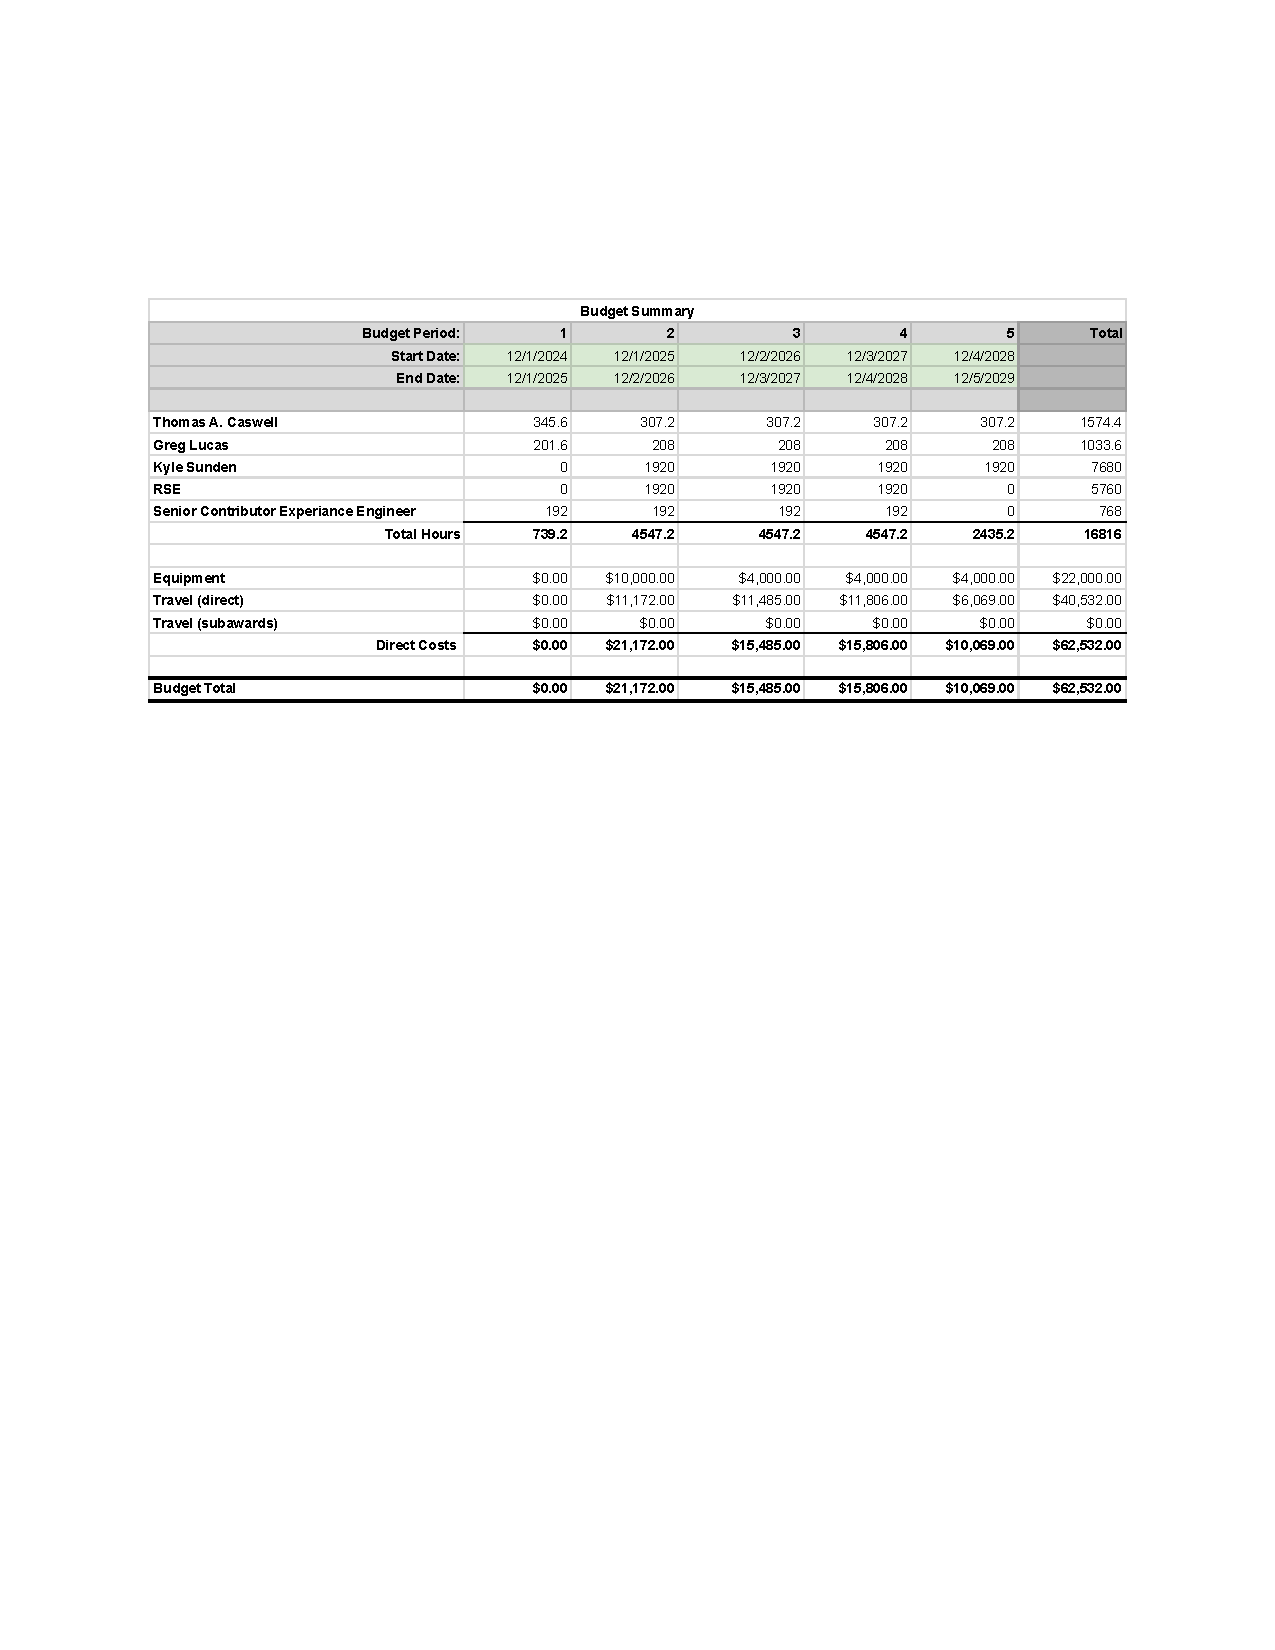
\includepdf[pagecommand={\subsection{Tabular Form}}]{detailed_budget}

\end{document}
